\documentclass[nojss]{jss} % nojss articlen sijaan

%\VignetteIndexEntry{gmvarkit: A Family of Mixture Vector Autoregressive Models in R}

%% HUOM: alla olevat uGMAR paperille
%% setwd("/Users/savi/Desktop/uGMARartikkeli/jss-article-rnw")
%% Sweave("uGMARpaper.Rnw")
%% tools::texi2pdf("uGMARpaper.tex")

%% -- LaTeX packages and custom commands ---------------------------------------

%% recommended packages
\usepackage{thumbpdf,lmodern}

%% another package (only for this demo article)
\usepackage{framed}

%% Packages added by the author
\usepackage{amsmath} % \align, etc.
\usepackage{amssymb} % \mathbb, etc.
\usepackage{mathtools} % matrix*: [c] centered, [l] left-aligned, [r] right-aligned

%% new custom commands
\newcommand{\class}[1]{`\code{#1}'}
\newcommand{\fct}[1]{\code{#1()}}
\newtheorem{condition}{Condition}
\newtheorem{proposition}{Proposition}


%% For Sweave-based articles about R packages:
%% need no \usepackage{Sweave}



%% -- Article metainformation (author, title, ...) -----------------------------

%% - \author{} with primary affiliation
%% - \Plainauthor{} without affiliations
%% - Separate authors by \And or \AND (in \author) or by comma (in \Plainauthor).
%% - \AND starts a new line, \And does not.
\author{Savi Virolainen\\ University of Helsinki}
\Plainauthor{Savi Virolainen}

%% - \title{} in title case
%% - \Plaintitle{} without LaTeX markup (if any)
%% - \Shorttitle{} with LaTeX markup (if any), used as running title
%%\title{A Short Demo Article: Regression Models for Count Data in \proglang{R}}
\title{gmvarkit: A Family of Mixture Vector Autoregressive Models in \proglang{R}}
\Plaintitle{gmvarkit: A Family of Mixture Vector Autoregressive Models in R}
\Shorttitle{A Family of Mixture Autoregressive Models in \proglang{R}}

\Abstract{
We describe the \proglang{R} package \pkg{gmvarkit}, which provides tools for estimating and analyzing the reduced form and structural Gaussian mixture vector autoregressive model, the Student's $t$ mixture vector autoregressive model, and the Gaussian and Student's $t$ mixture vector autoregressive model. These three models constitute an appealing family of mixture autoregressive models that we call the GSMVAR models. The model parameters are estimated with the method of maximum likelihood by running multiple rounds of a two-phase estimation procedure in which a genetic algorithm is used to find starting values for a gradient based method. For evaluating the adequacy of the estimated models, \pkg{gmvarkit} utilizes so-called quantile residuals and provides functions for graphical diagnostics as well as for calculating formal diagnostic tests. \pkg{gmvarkit} also enables to simulate from the GSMVAR processes, to forecast future values of the process using a simulation-based Monte Carlo method, and to estimate generalized impulse response functions as well as generalized forecast error variance decompositions.  We illustrate the use of \pkg{gmvarkit} with a quarterly series consisting of two U.S. variables: the percentage change of real GDP and the percentage change of GDP implicit price deflator. This brief manuscript is intended as a vignette only but it was created with the Journal of Statistical Software style.
}

%% - \Keywords{} with LaTeX markup, at least one required
%% - \Plainkeywords{} without LaTeX markup (if necessary)
%% - Should be comma-separated and in sentence case.
\Keywords{mixture vector autoregressive model, regime-switching, Gaussian mixture, Student's $t$ mixture}
\Plainkeywords{mixture vector autoregressive model, regime-switching, Gaussian mixture, Student's t mixture}

%% - \Address{} of at least one author
%% - May contain multiple affiliations for each author
%%   (in extra lines, separated by \emph{and}\\).
%% - May contain multiple authors for the same affiliation
%%   (in the same first line, separated by comma).
\Address{
  Savi Virolainen\\
  Faculty of Social Sciences\\
  University of Helsinki\\
  P. O. Box 17, FI-0014 University of Helsinki, Finland\\
  E-mail: \email{savi.virolainen@helsinki.fi}
}

\begin{document}


\section{Introduction}
\textbf{If you came to read this vignette because you have trouble with the estimation, see Section~\ref{sec:example_estim}. If you have in particular trouble with the estimation of structural models, see also Section~\ref{sec:estim_structural}.}

Linear vector autoregressive (VAR) model is a standard tool in time series econometrics. It can be employed to answer questions about the statistical relationships of different variables or to forecast future values of the process, for example. Structural VAR model allows to trace out the effects of economic shocks that have been identified by the researcher. With an appropriate choice of the autoregressive order $p$, a linear VAR is often able to filter out autocorrelation from the series very well. If the errors are assumed to follow an autoregressive conditional heteroskedasticity (ARCH) process, the model is also often able to adequately filter out conditional heteroskedasticity from the series.

In some cases, linear VAR models are not, however, capable to capture all the relevant characteristics of the series. This includes shifts in the mean or volatility, and changes in the autoregressive dynamics of the process. Such nonlinear features frequently occur in economic time series when the underlying data generating dynamics vary in time, for example, depending the specific state of the economy. Various types of time series models capable of capturing such regime-switching behavior have been proposed, one of them being the class of mixture models introduced by \cite{Le+Martin+Raftery:1996} and further developed by, among others, \cite{Kalliovirta+Meitz+Saikkonen:2015}, \cite{Kalliovirta+Meitz+Saikkonen:2015}, \cite{Meitz+Preve+Saikkonen:2021}, \cite{Virolainen:2020}, and \cite{Virolainen:2021, Virolainen2:2021}. Following the recent developments of \cite{Kalliovirta+Meitz+Saikkonen:2016}, \cite{Virolainen:2020}, and \cite{Virolainen2:2021}, we consider the Gaussian mixture vector autoregressive (GMVAR) model, the Student's $t$ mixture vector autoregressive (StMVAR) model, and the Gaussian and Student's $t$ mixture autoregressive (G-StMVAR) model. These three models constitute an appealing family of mixture vector autoregressive models that we call the GSMVAR models.

A GSMVAR process generates each observation from one of its mixture components, which are either conditionally homoskedastic linear Gaussian vector autoregressions or conditionally heteroskedastic linear Student's $t$ vector autoregressions. The mixture component that generates each observation is randomly selected according to the probabilities determined by the mixing weights that, for a $p$th order model, depend on the full distribution of the previous $p$ observations. Consequently, the regime-switching probabilities may depend on the level, variability, kurtosis, and temporal dependence of the past observations. The specific formulation of the mixing weights also leads to attractive theoretical properties such as ergodicity and full knowledge of the stationary distribution of $p+1$ consecutive observations.

This paper describes the \proglang{R} package \pkg{gmvarkit} providing a comprehensive set of easy-to-use tools for GSMVAR modeling, including unconstrained and constrained maximum likelihood (ML) estimation of the model parameters, quantile residual based model diagnostics, simulation from the processes, forecasting, estimation generalized impulse response function (GIRF) and generalized forecast error variance decomposition (GFEVD), and more. Both, reduced form and structural GSMVAR models are covered. The emphasis is on estimation, as it can, in our experience, be rather tricky. In particular, due to the endogenously determined mixing weights, the log-likelihood function has a large number of modes, and in large areas of the parameter space, the log-likelihood function is flat in multiple directions. The log-likelihood function's global maximum point is also frequently located very near the boundary of the parameter space. However, such near-the-boundary estimates often maximize the log-likelihood function for a rather technical reason, and it might be more appropriate to consider an alternative estimate based on the largest local maximum point that is clearly in the interior of the parameter space.

The model parameters are estimated by running multiple rounds of a two-phase estimation procedure in which a modified genetic algorithm is used to find starting values for a gradient based variable metric algorithm. Because of the multimodality of the log-likelihood function, some of the estimation rounds may end up in different local maximum points, thereby enabling the researcher to build models not only based on the global maximum point but also on the local ones. The estimated models can be conveniently examined with the \code{summary} and \code{plot} methods. For evaluating their adequacy, \pkg{gmvarkit} utilizes multivariate quantile residual diagnostics in the framework presented in \cite{Kalliovirta+Saikkonen:2010}, including graphical diagnostics as well as diagnostic tests that take into account uncertainty about the true parameter value. Forecasting is based on a Monte Carlo simulation method. For univariate modeling, we suggest using the CRAN distributed R package \pkg{uGMAR} \citep{uGMAR}.

The remainder of this paper is organized as follows. Section~\ref{sec:models} introduces the GSMVAR models and discusses some of their properties. Section~\ref{sec:estimation} discusses estimation of the model parameters. In particular, we discuss many important practical aspects of the estimation that might not be obvious researchers unfamiliar with (S)GSMVAR modeling. We also illustrates how the GSMVAR models can be estimated and examined with \pkg{gmvarkit} and how parameter constraints can be tested.  In Section~\ref{sec:qres}, we describe quantile residuals and demonstrate how they can be utilized to evaluate model adequacy in \pkg{gmvarkit}. Section~\ref{sec:impulseresponse} discusses impulse response analysis based on generalized impulse response functions and generalized forecast error variance decompositions. Section~\ref{sec:GSMVAR} shows how the GSMVAR models can be built with given parameter values. In Section~\ref{sec:simufore}, we first show how to simulate observations from a GSMVAR process, and then we illustrate how to forecast future values of a GSMVAR process with a simulation-based Monte Carlo method. Section~\ref{sec:summary} concludes and collects some useful functions in \pkg{gmvarkit} to a single table for convenience. Appendix~\ref{ap:propt} provides density functions and some properties of multivariate Gaussian and Student's $t$ distributions. Finally, Appendix~\ref{sec:qresexpr} derives closed form expressions for the multivariate quantile residuals of the GSMVAR models.

Throughout this paper, we illustrate the use of \pkg{gmvarkit} with a quarterly series consisting of two U.S. variables: the percentage change of real GDP and the percentage change of GDP implicit price deflator, covering the period from 1959Q1 to 2019Q4. We deploy the notation $n_d(\boldsymbol{\mu},\boldsymbol{\Gamma})$ for the $d$-dimensional normal distribution with mean $\boldsymbol{\mu}$ and (positive definite) covariance matrix $\boldsymbol{\Gamma}$, and $t_d(\boldsymbol{\mu},\boldsymbol{\Gamma},\nu)$ for the $d$-dimensional $t$-distribution with mean $\boldsymbol{\mu}$, (positive definite) covariance matrix $\boldsymbol{\Gamma}$, and $\nu>2$ degrees of freedom. The corresponding density functions are denoted as $n_d(\cdot;\boldsymbol{\mu},\boldsymbol{\Gamma})$ and $t_d(\cdot;\boldsymbol{\mu},\boldsymbol{\Gamma},\nu)$, respectively. By $\boldsymbol{1}_p=(1,...,1)$ ($p \times 1$), we denote $p$-dimensional vector of ones. Finally, $\otimes$ denotes Kronecker product.

\section{Models}\label{sec:models}
This section introduces the GMVAR model \citep{Kalliovirta+Meitz+Saikkonen:2016}, the StMVAR model \citep{Virolainen2:2021}, and the G-StMVAR model \citep{Virolainen2:2021}, a family of mixture vector autoregressive models that we call the GSMVAR models. First, we define the component processes of the GSMVAR models - linear VARs based on either Gaussian or Student's $t$ distribution. Then, we introduce the reduced form GSMVAR models. For brevity, we only give the definition of the more general G-StMVAR model but explain how the GMVAR and StMVAR models are obtained as special cases of it, namely, by taking all the component models to be of either Gaussian or Student's $t$ type. After defining the reduced form GSMVAR model, we introduce structural version of the models incorporating statistically identified structural shocks. Identification of the shocks is also briefly discussed.

\section{Linear Gaussian and Student's $t$ vector autoregressions}
To develop theory and notation, consider first the component processes of the Gaussian and Student's $t$ mixture vector autoregressive models. For a $p$th order linear Gaussian or Student's $t$ vector autoregression $z_t$, we have
\begin{equation}\label{eq:gaussianvar}
z_t = \phi_{0} + \sum_{i=1}^pA_iz_{t-1} + \Omega_t^{1/2}\varepsilon_t, \quad \varepsilon\sim IID(0,I_d),
\end{equation}
where $\Omega_t^{1/2}$ is a symmetric square root matrix of the positive definite $(d\times d)$ covariance matrix $\Omega_t$, and $\phi_0\in\mathbb{R}^d$. The $(d \times d)$ autoregression matrices are assumed to satisfy $\boldsymbol{A}_p \equiv [A_1:...:A_p]\in\mathbb{S}^{d\times dp}$, where
\begin{equation}\label{eq:statreg}
\mathbb{S}^{d\times dp}= \lbrace [A_1:...:A_p]\in\mathbb{R}^{d\times dp}: \det(I_d - \sum_{i=1}^pA_iz^i)\neq 0 \ \text{for} \ |z|\leq 1 \rbrace
\end{equation}
defines the usual stability condition of a linear vector autoregression.

In the case of Gaussian VAR, the errors \varepsilon_t are assumed standard normal distributed and the covariance matrices $\Omega_t=\Omega$ are time invariant. Denoting $\boldsymbol{z}_t=(z_t,...,z_{t-p+1})$ and $\boldsymbol{z}_t^{+}=(z_t,\boldsymbol{z}_{t-1})$, it is well known that with IID Gaussian error process the stationary solution to (\ref{eq:gaussianvar}) satisfies
\begin{align}\label{eq:gausdist}
\begin{aligned}
\boldsymbol{z}_t & \sim n_{dp}(\boldsymbol{1}_p\otimes\mu,\Sigma_{p}) \\
\boldsymbol{z}^{+}_t & \sim n_{d(p+1)}(\boldsymbol{1}_{p+1}\otimes\mu,\Sigma_{p+1}) \\
z_t|\boldsymbol{z}_{t-1} & \sim n_d(\phi_{0} + \boldsymbol{A}_p\boldsymbol{z}_{t-1}, \Omega),
 \end{aligned}
\end{align}
where the last line defines the conditional distribution of $z_t$ given $\boldsymbol{z}_{t-1}$.  Denoting by $\Sigma(h)$ the lag $h$ ($h=0,\pm 1, \pm 2,...$) autocovariance matrix of $z_t$, the quantities $\mu,\Sigma_p,\Sigma_1,\Sigma_{1p},\Sigma_{p+1}$ are given as \cite[see, e.g.,][pp.  23,  28-29]{Lutkepohl:2005}
\begin{align}\label{eq:gausquantities}
\begin{aligned}
\mu = & (I_d - \sum_{i=1}^pA_i)^{-1}\phi_0 & (d\times 1) \\
\text{vec}(\Sigma_p) = & (I_{(dp)^2} - \boldsymbol{A}\otimes\boldsymbol{A})^{-1}\text{vec}(\boldsymbol{\Omega}) & ((dp)^2\times 1)  \\
\Sigma_1 = & \Sigma(0) %= A_1\Sigma(1)'+\cdots + A_p\Sigma(p)'+\Omega
& (d\times d) \\
\Sigma(p) = & A_1\Sigma(p - 1) + \cdots + A_p\Sigma(0) & (d\times d) \\
\Sigma_{1p} = & [\Sigma(1):...:\Sigma(p-1):\Sigma(p)] = \boldsymbol{A}_p\Sigma_p & (d\times dp) \\
\Sigma_{p+1} = &
\begin{bmatrix}
\Sigma_1       & \Sigma_{1p} \\
\Sigma_{1p}' & \Sigma_p
\end{bmatrix}
& (d(p+1) \times d(p+1))
\end{aligned}
\end{align}
where
\begin{align}\label{eq:gausmatrices}
\begin{aligned}
\Sigma_p = &
\underset{(dp\times dp)}{\begin{bmatrix}
\Sigma(0) &  \Sigma(1) & \cdots & \Sigma(p-1) \\
\Sigma(-1) &  \Sigma(0) & \cdots & \Sigma(p-2) \\
\vdots        &   \vdots   & \ddots & \vdots  \\
\Sigma(-p+1) &  \Sigma(-p+2) & \cdots & \Sigma(0) \\
\end{bmatrix}},
\\
\boldsymbol{A} = &
\underset{(dp\times dp)}{\begin{bmatrix}
A_1 & A_2 & \cdots & A_{p-1} & A_p \\
I_d  & 0     & \cdots & 0            & 0 \\
0     & I_d  &             & 0            & 0 \\
\vdots &   & \ddots & \vdots    & \vdots \\
0     & 0     & \hdots & I_d         & 0
\end{bmatrix}},
\ \ \text{and} \ \
\boldsymbol{\Omega} =
\underset{(dp\times dp)}{\begin{bmatrix}
\Omega & 0 & \cdots & 0  \\
0            & 0 & \cdots & 0   \\
\vdots    &  \vdots & \ddots & \vdots \\
0            & 0 & \hdots &  0
\end{bmatrix}}.
\end{aligned}
\end{align}

\cite{Virolainen2:2021} shows that there are exists conditionally heteroskecastic Student's $t$ vector autoregressions with distributional properties similar to the Gaussian VARs. Using the notation described above, these Student's $t$ VARs are obtained by assuming $\varepsilon_t\sim t_d(0,I_d,\nu + dp)$ and
\begin{equation}
\Omega_t = \frac{\nu - 2 + (\boldsymbol{z} - \boldsymbol{1}_p\otimes\mu)'\Sigma_p^{-1}(\boldsymbol{z} - \boldsymbol{1}_p\otimes\mu)}{\nu - 2 + dp}\Omega.\label{eq:convarlinear}
\end{equation}
These Student's $t$ VARs are stationary and satisfy \citep[Theorem 1]{Virolainen2:2021}
\begin{align}\label{eq:studentdist}
\begin{aligned}
\boldsymbol{z}_t & \sim t_{dp}(\boldsymbol{1}_p\otimes\mu,\Sigma_{p},\nu) \\
\boldsymbol{z}^{+}_t & \sim t_{d(p+1)}(\boldsymbol{1}_{p+1}\otimes\mu,\Sigma_{p+1},\nu) \\
z_t|\boldsymbol{z}_{t-1} & \sim t_d(\phi_{0} + \boldsymbol{A}_p\boldsymbol{z}_{t-1}, \Omega_t, \nu + dp),
 \end{aligned}
\end{align}
The conditional variance (\ref{eq:convarlinear}) consists of a constant covariance matrix that is multiplied by a time-varying scalar that depends on the quadratic form of the preceding $p$ observations through the autoregressive parameters.  In this sense,  the model has a ‘VAR($p$)–ARCH($p$)’ representation,  but the ARCH type conditional variance is not as general as in the conventional multivariate ARCH process \citep[e.g., ][Section 16.3]{Lutkepohl:2005} that allows the entries of the conditional covariance matrix to vary relative to each other.

We refer often to the linear Gaussian VARs as GMVAR type, because they are similar to the component processes of the GMVAR model \citep{Kalliovirta+Meitz+Saikkonen:2016}. Likewise, we often refer to the linear Student's $t$ VARs as StMVAR type, because they are similar to the component processes of the StMVAR model \citep{Virolainen2:2021}. The G-StMVAR model \citep{Virolainen2:2021} incorporates both types of component processes. Because the GMVAR are StMVAR model are obtained as special cases of the G-StMVAR model by assuming that all the component processes are either GMVAR or StMVAR type, we will only give the definition of the more general G-StMVAR model.

\section{Gaussian and Student's $t$ mixture vector autoregressive model}
Let $y_t$ $(t=1,2,...)$ be the real valued time series of interest, and let $\mathcal{F}_{t-1}$ denote $\sigma$-algebra generated by the random variables $\lbrace y_s, s<t \rbrace$. In a G-StMVAR model \citep{Virolainen2:2021} with autoregressive order $p$ and $M$ mixture components (or regimes),  the observations $y_t$ are assumed to be generated by
\begin{align}
y_t = & \sum_{m=1}^Ms_{m,t}(\mu_{m,t} + \Omega_{m,t}^{1/2}\varepsilon_{m,t}), \label{eq:def} \\
\mu_{m,t} = & \phi_{m,0} + \sum_{i=1}^pA_{m,i}y_{t-i},\label{eq:mu_mt}
\end{align}
where the following conditions hold.
%
\begin{condition}\label{cond:def}
\
\begin{enumerate}
\item For $m=1,...,M_1\leq M$,  the random vectors $\varepsilon_{m,t}$ are IID $n_d(0, I_d)$ distributed,  and for $m=M_1+1,..., M$, they are IID $t_d(0, I_d,\nu_m + dp)$ distributed. For all $m$,  $\varepsilon_{m,t}$ are independent of $\mathcal{F}_{t-1}$.
\item For each $m=1,...,M$‚ $\phi_{m,0}\in\mathbb{R}^d$,  $\boldsymbol{A}_{m,p} \equiv [A_{m,1}:...:A_{m,p}]\in\mathbb{S}^{d\times dp}$ (the set $\mathbb{S}^{d\times dp}$ is defined in (\ref{eq:statreg})),  and $\Omega_m$ is positive definite.  For $m=1,...,M_1$,  the conditional covariance matrices are constants, $\Omega_{m,t}=\Omega_m$.  For $m=M_1+1,...,M$,  the conditional covariance matrices $\Omega_{m,t}$ are as in (\ref{eq:convarlinear}), except that $\boldsymbol{z}$ is replaced with $\boldsymbol{y}_{t-1}=(y_{t-1},...,y_{t-p})$ and the regime specific parameters $\phi_{m,0}$, $\boldsymbol{A}_{m,p}$,$\Omega_m$,$\nu_m$ are used to define the quantities therein.  For $m=M_1+1,...,M$, also  $\nu_m>2$.
\item The unobservable regime variables $s_{1,t},...,s_{M,t}$ are such that at each $t$, exactly one of them takes the value one and the others take the value zero according to the conditional probabilities expressed in terms of the ($\mathcal{F}_{t-1}$-measurable) mixing weights $\alpha_{m,t}\equiv Pr(s_{m,t}=1|\mathcal{F}_{t-1})$ that satisfy $\sum_{m=1}^M\alpha_{m,t}=1$.
\item Conditionally on $\mathcal{F}_{t-1}$,  $(s_{1,t},...,s_{M,t})$ and $\varepsilon_{m,t}$ are assumed independent.
\end{enumerate}
\end{condition}

The conditions $\nu_m>2$ are made to ensure the existence of second moments.  This definition implies that the G-StMVAR model generates each observation from one of its mixture components, linear Gaussian or Student's $t$ vector autoregression discussed in Section~\ref{sec:linvar}, and that the mixture component is selected randomly according to the probabilities given by the mixing weights $\alpha_{m,t}$. The first $M_1$ mixture components are assumed to be linear Gaussian VARs,  and the last $M_2\equiv M - M_1$ mixture components are assumed to be linear Student's $t$ VARs.  If all the component processes are Gaussian VARs ($M_1=M$),  the G-StMVAR model reduces to the GMVAR model of \cite{Kalliovirta+Meitz+Saikkonen:2016}.  If all the component processes are Student's $t$ VARs ($M_1=0$),  we refer to the model as the StMVAR model. %Sometimes we refer to the Gaussian mixture components as GMVAR type and to the Student's $t$ mixture components as StMVAR type.

The definition (\ref{eq:def}),  (\ref{eq:mu_mt}), and Condition~\ref{cond:def} leads to a model in which the conditional density function of $y_t$ conditional on its past, $\mathcal{F}_{t-1}$,  is given as
\begin{equation}\label{eq:conddist}
f(y_t|\mathcal{F}_{t-1}) = \sum_{m=1}^{M_1}\alpha_{m,t}n_d(y_t;\mu_{m,t},\Omega_{m}) +  \sum_{m=M_1+1}^M\alpha_{m,t}t_d(y_t;\mu_{m,t},\Omega_{m,t},\nu_m+dp).
\end{equation}
The conditional densities $n_d(y_t;\mu_{m,t},\Omega_{m,t})$ are obtained from (\ref{eq:gausdist}),  whereas $t_d(y_t;\mu_{m,t},\Omega_{m,t},\nu_m+dp)$ are obtained from \citet[Theorem 1]{Virolainen2:2021}. The explicit expressions of the density functions are given in Appendix~\ref{ap:propt. To fully define the G-StMVAR model, it is then left to specify the mixing weights $\alpha_{m,t}$.

The mixing weights are defined as as weighted ratios of the component process stationary densities corresponding to the previous $p$ observations. In order to formally specify the mixing weights,  we first define the following function for notational convenience. Let
\begin{equation}\label{eq:d_mdp}
d_{m,dp}(\boldsymbol{y};\mathbf{1}_p\otimes\mu_m,\Sigma_{m,p},\nu_m)=
\left\{\begin{matrix*}[l]
 n_{dp}(\boldsymbol{y};\mathbf{1}_p\otimes\mu_m,\Sigma_{m,p}), & \text{when} \ m \leq M_1, \\
 t_{dp}(\boldsymbol{y};\mathbf{1}_p\otimes\mu_m,\Sigma_{m,p},\nu_m), & \text{when} \ m > M_1,
\end{matrix*}\right.
\end{equation}
where the $dp$-dimensional densities $n_{dp}(\boldsymbol{y};\mathbf{1}_p\otimes\mu_m,\Sigma_{m,p})$ and $t_{dp}(\boldsymbol{y};\mathbf{1}_p\otimes\mu_m,\Sigma_{m,p},\nu_m)$ correspond to the stationary distribution of the $m$th component process (given in equations (\ref{eq:gausdist}) and (\ref{eq:studentdist})).  Denoting $\boldsymbol{y}_{t-1}=(y_{t-1},...,y_{t-p})$, the mixing weights of the G-StMVAR model are defined as
\begin{equation}\label{eq:alpha_mt}
\alpha_{m,t} = \frac{\alpha_md_{m,dp}(\boldsymbol{y}_{t-1};\mathbf{1}_p\otimes\mu_m,\Sigma_{m,p},\nu_m)}{\sum_{n=1}^M \alpha_n d_{n,dp}(\boldsymbol{y}_{t-1};\mathbf{1}_p\otimes\mu_n,\Sigma_{n,p},\nu_n)},
\end{equation}
where $\alpha_m\in (0,1)$, $m=1,...,M$, are mixing weights parameters assumed to satisfy $\sum_{m=1}^M\alpha_m = 1$,  $\mu_m = (I_d - \sum_{i=1}^pA_{m,i})^{-1}\phi_{m,0}$,  and covariance matrix $\Sigma_{m,p}$ is given in (\ref{eq:gausquantities}) and (\ref{eq:gausmatrices}) but using the regime specific parameters to define the quantities therein.

Because the mixing weights are weighted component process's stationary densities corresponding to the previous $p$ observations,  an observation is more likely to be generated from a regime with higher relative weighted likelihood.  This is a convenient feature for forecasting but it also allows the researcher to associate specific characteristics to different regimes.  Moreover,  it turns out that this specific formulation of the mixing weights leads to attractive properties such as full knowledge of the stationary distribution of $p+1$ consecutive observations and ergodicity of the process. Specifically,  $\boldsymbol{y}_t=(y_t,...,y_{t-p+1})$ has stationary distribution that is characterized by the density \citep[Theorem 2]{Virolainen2:2021}
\begin{equation}
f(\boldsymbol{y}) = \sum_{m=1}^M\alpha_m n_{dp}(\boldsymbol{y};\boldsymbol{1}_p\otimes\mu_{m},\Sigma_{m,p}) + \sum_{m=M_1+1}^M\alpha_mt_{dp}(\boldsymbol{y};\boldsymbol{1}_p\otimes\mu_{m},\Sigma_{m,p},\nu_m).
\end{equation}

\pkg{gmvarkit} collects the parameters of a G-StMVAR model to the $((M(d + d^2p + d(d+1)/2 + 2) - M_1 - 1)\times 1)$ vector $\boldsymbol{\theta}=(\boldsymbol{\vartheta}_1,...,\boldsymbol{\vartheta}_M,\alpha_1,...,\alpha_{M-1},\boldsymbol{\nu})$,  where $\boldsymbol{\vartheta}_m=(\phi_{m,0},vec(\boldsymbol{A}_{m,p}),vech(\Omega_m))$ and $\boldsymbol{\nu}=(\nu_{M_1+1},...,\nu_M)$.  The last mixing weight parameter $\alpha_M$ is not parametrized because it is obtained from the restriction $\sum_{m=1}^M \alpha_m = 1$.  A G-StMVAR model with autoregressive order $p$,  and $M_1$ GMVAR type and $M_2$ StMVAR type mixture components is referred to as G-StMVAR($p,M_1,M_2$) model, whenever the order of the model needs to be emphasized. If the model imposes constraints, the parameter vector is different. For details, see the documentation.


\section{Structural G-StMVAR model}\label{sec:structural_model}
We write the structural G-StMVAR model \citep{Virolainen2:2021} as
\begin{equation}
y_t = \sum_{m=1}^Ms_{m,t}(\phi_{m,0}+\sum_{i=1}^pA_{m,i}y_{t-i}) + B_te_t
\end{equation}
and
\begin{equation}
u_t\equiv B_te_t =
\left\lbrace\begin{matrix}
u_{1,t}\sim n_d(0,\Omega_{1,t}) & \text{if} & s_{1,t}=1 & (\text{with probability } \alpha_{1,t}) \\
\vdots & & & \\
u_{M_1,t}\sim n_d(0,\Omega_{M_1,t}) & \text{if} & s_{M_1,t}=1 & (\text{with probability } \alpha_{M_1,t}) \\
u_{M_1+1,t}\sim t_d(0,\Omega_{M_1+1,t},\nu_m + dp) & \text{if} & s_{M_1+1,t}=1 & (\text{with probability } \alpha_{M_1,t}) \\
\vdots & & & \\
u_{M,t}\sim t_d(0,\Omega_{M,t},\nu_m + dp) & \text{if} & s_{M,t}=1 & (\text{with probability } \alpha_{M,t})
\end{matrix}\right.
\end{equation}
where the probabilities are expressed conditionally on $\mathcal{F}_{t-1}$ and $e_t$ $(d \times 1)$ in an orthogonal structural error.  For the GMVAR type regimes, $m=1,...,M_1$‚ $\Omega_{m,t}=\Omega_m$.  For the StMVAR type regimes,  $m=M_1+1,...,M$,  $\Omega_{m,t}=\sigma_{m,t}^2\Omega_m$, where
\begin{equation}\label{eq:sigma_mt}
\sigma_{m,t}^2 = \frac{\nu_m - 2 + (\boldsymbol{y}_{t-1} - \boldsymbol{1}_p\otimes\mu_m)'\Sigma_{m,p}^{-1}(\boldsymbol{y}_{t-1} - \boldsymbol{1}_p\otimes\mu_m)}{\nu_m - 2 + dp}.
\end{equation}
The invertible $(d\times d)$ "B-matrix" $B_t$, which governs the contemporaneous relations of the shocks, is time-varying and a function of $y_{t-1},..., y_{t-p}$. With a particular choice of $B_t$,  the conditional covariance matrix of the structural error can be normalized to an identity matrix. Consequently,  a constant sized structural shock will be amplified according to the conditional variance of the reduced form error, thereby reflecting the specific state of the economy.

We have $\Omega_{u,t}\equiv\text{Cov}(u_t|\mathcal{F}_{t-1})=\sum_{m=1}^{M_1}\alpha_{m,t}\Omega_m + \sum_{m=M_1+1}^{M}\alpha_{m,t}\sigma_{m,t}^2\Omega_m$,  while the conditional covariance matrix of the structural error $e_t=B_t^{-1}u_t$ (which are not IID but are martingale differences and therefore uncorrelated) is obtained as
\begin{equation}
\text{Cov}(e_t|\mathcal{F}_{t-1})=\sum_{m=1}^{M_1}\alpha_{m,t}B_t^{-1}\Omega_mB_t'^{-1} + \sum_{m=M_1+1}^{M}\alpha_{m,t}\sigma_{m,t}^2B_t^{-1}\Omega_mB_t'^{-1}.
\end{equation}
Therefore, we need to choose the B-matrix so that the structural shocks are orthogonal regardless of which regime they come from.

We employ the following decomposition to simultaneously diagonalize all the error term covariance matrices:
\begin{equation}\label{eq:omega_decomp}
\Omega_m = W\Lambda_mW',  \ \ m=1,...,M,
\end{equation}
where the diagonal of $\Lambda_m = \text{diag}(\lambda_{m1},...,\lambda_{md})$,  $\lambda_{mi}>0$ $(i=1,...,d)$,  contains the eigenvalues of the matrix $\Omega_m\Omega_1^{-1}$ and the columns of the nonsingular $W$ are the related eigenvectors (that are the same for all $m$ by construction).  When $M=2$,  the decomposition (\ref{eq:omega_decomp}) always exists, but for $M\geq 3$ its existence requires that the matrices share the common eigenvectors in $W$.  This is, however, testable.

\citet[Proposition 1]{Lanne+Lutkepohl+Maciejowska:2010} show that for a given ordering of the eigenvalues, $W$ is unique apart from changing all signs a column, as long as for all $i\neq j\in \lbrace 1,...,d \rbrace$ there exists an $m\in\lbrace 2,...,M \rbrace$ such that $\lambda_{mi}\neq\lambda_{mj}$ (for $m=1$,  $\Lambda_m=I_d$ and $\lambda_{m1}=\cdots = \lambda_{md}=1$).  A locally unique B-matrix that amplifies a constant sized structural shock according to the conditional variance of the reduced form error is therefore obtained as
\begin{equation}\label{eq:B-matrix}
B_t = W(\sum_{m=1}^{M_1}\alpha_{m,t}\Lambda_m + \sum_{m=M_1 + 1}^{M}\alpha_{m,t}\sigma_{m,t}^2\Lambda_m)^{1/2}.
\end{equation}
Since $B_t^{-1}\Omega_mB_t'^{-1}=\Lambda_m(\sum_{n=1}^{M_1}\alpha_{n,t}\Lambda_n + \sum_{n=M_1+1}^M\alpha_{n,t}\sigma_{n,t}^2\Lambda_n)^{-1}$,  the B-matrix (\ref{eq:B-matrix}) simultaneously diagonalizes $\Omega_{1},...,\Omega_{M}$, and $\Omega_{u,t}$ (and thereby also $\Omega_{1,t},...,\Omega_{M,t}$) for each $t$ so that $\text{Cov}(e_t|\mathcal{F}_{t-1}) = I_d$.


\subsection{Identification of the structural shocks}
With the decomposition (\ref{eq:omega_decomp}) of $\Omega_1,...,\Omega_M$ and the B-matrix (\ref{eq:B-matrix}),  a statistical identification of the shocks is achieved as long as each pair of the eigenvalues is distinct for some $m$.  In order to identify structural shocks with economic interpretations,  they need to be uniquely related to the economic shocks through the constraints on the B-matrix (or equally $W$) that only the shock of interest satisfies. \citet[Proposition 1]{Virolainen:2020} gives formal conditions for global identification of any subset of the shocks when the relevant pairs eigenvalues are distinct in some regime.  He also derives conditions for globally identifying some of the shocks when one of the relevant pairs of the eigenvalues is identical in all regimes.  For convenience,  we repeat the conditions in the former case below,  but in the latter case,  we refer to \citet[Proposition 2]{Virolainen:2020}.
\begin{proposition}\label{prop:ident1}
Suppose $\Omega_m = W\Lambda_mW'$,  $m=1,...,M$, where the diagonal of $\Lambda = \text{diag}(\lambda_{m1},...,\lambda_{md})$,  $\lambda_{mi}>0$ $(i=1,...,d)$,  contains the eigenvalues of the matrix $\Omega_m\Omega_1^{-1}$ and the columns of the nonsingular $W$ are the related eigenvectors.  Then,  the last $d_1$ structural shocks are uniquely identified if
\begin{enumerate}
\item for all $j>d-d_1$ and $i \neq j$ there exists an $m\in\lbrace 2,...,M\rbrace$ such that $\lambda_{mi}\neq \lambda_{mj}$,\label{cond:lambdadif}
\item the columns of $W$ in a way that for all $i\neq j > d - d_1$, the $i$th column cannot satisfy the constraints of the $j$th column as is nor after changing all signs in the $i$th column, and\label{cond:Wconstraints}
\item there is at least one (strict) sign constraint in each of the last $d_1$ columns of $W$. \label{cond:Wsign}
\end{enumerate}
\end{proposition}
Condition \ref{cond:Wsign} fixes the signs in the last $d_1$ columns of $W$,  and therefore the signs of the instantaneous effects of the corresponding shocks.  However,  since changing the signs of the columns is effectively the same as changing the signs of the corresponding shocks, and the structural shock has a distribution that is symmetric about zero,  this condition is not restrictive.  The assumption that the last $d_1$ shocks are identified is not restrictive either,  as one may always reorder the structural shocks accordingly.

For example, if $d=3$, $\lambda_{m1}\neq\lambda_{m3}$ for some $m$, and $\lambda_{m2}\neq\lambda_{m3}$ for some $m$, the third structural shock can be identified with the following constraints:
\begin{equation}
B_t=\begin{bmatrix}
* & * & *    \\
+ & + &  - \\
+ & + & + \\
\end{bmatrix}
\ \text{or} \
\begin{bmatrix}
- & * & + \\
- & + & -  \\
* & + & + \\
\end{bmatrix}
\ \text{or} \
\begin{bmatrix}
+ & 0 & -  \\
* & * & *  \\
+ & * & + \\
\end{bmatrix}
\end{equation}
and so on, where $"*"$ signifies that the element is not constrained, $"+"$ denotes strict positive and $"-"$ a strict negative sign constraint, and $"0"$ means that the element is constrained to zero. Because imposing zero or sign constraints on $W$ equals to placing them on $B_t$, they may be justified economically. Furthermore, besides a single sign constraint in each column, the constraints are over-identifying and can thus be also justified statistically. Sign constraints, however, don't reduce the dimension of the parameter space, making some of the measures such as the conventional likelihood ratio test and information criteria unsuitable for testing them. Quantile residual diagnostics, on the other hand, can be used to evaluate how well the restricted model is able to encapsulate the statistical properties of the data compared to the unrestricted alternative.

If condition~\ref{cond:lambdadif} of Proposition~\ref{prop:ident1} is strengthened to state that for all $i\neq j$ there exists an $m\in\lbrace 2,...,M\rbrace$ such that $\lambda_{mi}\neq \lambda_{mj}$,  the model is statistically identified even though only the last $d_1$ structural shocks have been identified with the proposition.  Consequently,  the constraints imposed in condition \ref{cond:Wconstraints} become testable.  If it cannot be assumed that all the pairs of the eigenvalues are distinct in some regime,  then the testing problem is nonstandard and the conventional asymptotic distributions of likelihood ratio and Wald test statistics become unreliable.  Note,  however, that since placing zero or sign constraints on $W$ equals to placing them on the B-matrix (\ref{eq:B-matrix}),  the constraints imposed in condition \ref{cond:Wconstraints} can be justified economically as usual.


\section{Estimation and model selection}\label{sec:estimation}

\subsection{Log-likelihood function}\label{sec:loglik}
\pkg{gmvarkit} employs the method of maximum likelihood (ML) for estimating the parameters of the G-StMVAR model. Even the exact log-likelihood function is available, as we have established the stationary distribution of the process in Theorem~\ref{thm:statdist}.  Suppose the observed time series is $y_{-p+1},...,y_0,y_1,...,y_T$ and that the initial values are stationary.  Then, the log-likelihood function of the G-StMVAR model takes the form
\begin{equation}\label{eq:loglik1}
L(\boldsymbol{\theta})=\log\left(\sum_{m=1}^M\alpha_m d_{m,dp}(\boldsymbol{y}_0;\boldsymbol{1}_p\otimes\mu_m,\Sigma_{m,p},\nu_m) \right) + \sum_{m=1}^M l_t(\boldsymbol{\theta}),
\end{equation}
where $d_{m,dp}(\cdot;\boldsymbol{1}_p\otimes\mu_m,\Sigma_{m,p},\nu_m)$ is defined in (\ref{eq:d_mdp}) and
\begin{equation}\label{eq:loglik2}
l_t(\boldsymbol{\theta}) = \log\left(\sum_{m=1}^{M_1}  \alpha_{m,t}n_d(y_t;\mu_{m,t},\Omega_{m})  + \sum_{m=M_1 + 1}^M  \alpha_{m,t}t_d(y_t;\mu_{m,t},\Omega_{m,t},\nu_m + dp  ) \right).
\end{equation}
If stationarity of the initial values seems unreasonable,  one can condition on the initial values and base the estimation on the conditional log-likelihood function, which is obtained by dropping the first term on the right hand side of (\ref{eq:loglik1}).

\citet[Theorem 3]{Virolainen2:2021} shows that the ML estimator of the G-StMVAR model is strongly consistent and has the conventional high-level conditions. In the case of a GMVAR model ($M_1=M$), however, establishing asymptotic normality of the ML estimator requires less unverified assumptions \cite[Theorem 3]{Kalliovirta+Meitz+Saikkonen:2016}.

If there are two regimes in the model ($M=2$),  the structural G-StMVAR model is obtained from estimated reduced form model by decomposing the covariance matrices $\Omega_1,...,\Omega_M$ as in (\ref{eq:omega_decomp}).  If $M\geq 3$ or overidentifying constraints are imposed on $B_t$ through $W$,  the model can be reparametrized with $W$ and $\Lambda_m$ ($m=2,...,M$) instead of $\Omega_1,...,\Omega_M$,  and the log-likelihood function can be maximized subject to the new set of parameters and constraints.\footnote{Namely,  instead of constraining $vech(\Omega_1),...,vech(\Omega_M)$ so that $\Omega_1,...,\Omega_M$ are positive definite,  we impose the constraints $\lambda_{mi}>0$ for all $m=2,...,M$ and $j=1,...,d$.} In this case, the decomposition (\ref{eq:omega_decomp}) is plugged in to the log-likelihood function and $vech(\Omega_1),...,vech(\Omega_M)$ are replaced with $vec(W)$ and $\boldsymbol{\lambda}_2,...,\boldsymbol{\lambda}_M$ in the parameter vector $\boldsymbol{\theta}$,  where $\boldsymbol{\lambda}_m=(\lambda_{m1},...,\lambda_{md})$.


\subsection{Two-phase estimation procedure}\label{sec:estimscheme}
Finding the ML estimate amounts maximizing the log-likelihood function (\ref{eq:loglik1}) (and (\ref{eq:loglik2})) over a high dimensional parameter space satisfying the constraints summarized in Assumption~\ref{as:mle}.  Due to the complexity of the log-likelihood function, numerical optimization methods are required.  The maximization problem can, however, be challenging in practice.  This is particularly due to the mixing weights' complex dependence on the preceding observations,  which induces a large number of modes to the surface of the log-likelihood function, and large areas to the parameter space where it is flat in multiple directions.  Also, the popular EM algorithm \citep{Redner+Walker:1984} is virtually useless here,  as at each maximization step one faces a new optimization problem that is not much simpler than the original one.  Following \cite{Meitz+Preve+Saikkonen2:2018, Meitz+Preve+Saikkonen:2021} and \cite{Virolainen:2021, uGMAR}, we therefore employ a two-phase estimation procedure in which a genetic algorithm is used to find starting values for a gradient based method.

The genetic algorithm in \pkg{gmvarkit} is, at core, mostly based on the description by \cite{Dorsey+Mayer:1995} but several modifications have been deployed to improve its performance. The modifications include the ones proposed by \cite{Patnaik+Srinivas:1994} and \cite{Smith+Dike+Stegmann:1995} as well as further adjustments that take into account model specific issues related to the mixing weights' dependence on the preceding observations. For a more detailed description of the genetic algorithm and its modifications, see \citet[Appendix A]{Virolainen:2021}, where the genetic algorithm is discussed in the univariate context. After running the genetic algorithm, the estimation is finalized with a variable metric algorithm \cite[algorithm 21, implemented by \citealp{R}]{Nash:1990} using central difference approximation for the gradient of the log-likelihood function.

\subsection{Examples of unconstrained estimation}\label{sec:example_estim}
In this section, we demonstrate how to estimate GSMVAR models with \pkg{gmvarkit} and provide several examples in order to illustrate various frequently occurring situations. In addition to the ordinary estimation, we particularly show how a GSMVAR model can be built based on a local-only maximum point when the ML estimate seems unreasonable. We also consider the estimation of the appropriate G-StMVAR model when the estimated StMVAR model contains overly large degrees of freedom estimates \citep[see the related discussion in][]{Virolainen2:2021}. In the examples, we only consider $p=1$ models for simplicity and because then the code outputs fit in the margins better, estimation times are shorter, etc. This order may not be best in the modeling perspective, however.

In \pkg{gmvarkit}, the GSMVAR models are defined as class \code{gsmvar} S3 objects, which can be created with given parameter values using the constructor function \code{GSMVAR} (see Section~\ref{sec:GSMVAR}) or by using the estimation function \code{fitGSMVAR}, which estimates the parameters and then builds the model. For estimation, \code{fitGSMVAR} needs to be supplied with a univariate time series and the arguments specifying the model. The necessary arguments for specifying the model include the autoregressive order \code{p}, the number of mixture components \code{M}, and \code{model}, which should be either \code{"GMVAR"}, \code{"StMVAR"}, or \code{"G-StMVAR"}. For GMVAR and StMVAR models, the argument \code{M} is a positive integer, whereas for the G-StMVAR model it is a length two numeric vector specifying the number of GMVAR type regimes in the first element and the number of StMVAR type regimes in the second.

Additional arguments may be supplied to \code{fitGSMVAR} in order to specify, for example, whether the exact log-likelihood function should be used instead of the conditional one (\code{conditional}), how many estimation rounds should be performed (\code{ncalls}), and how many central processing unit (CPU) cores should be used in the estimation (\code{ncores}). Some of the estimation rounds may end up in local-only maximum points or saddle points, but reliability of the estimation results can be improved by increasing the number of estimation rounds. A large number of estimation rounds may be required particularly when the number of mixture components is large, as the surface of the log-likelihood function becomes increasingly more challenging. It is also possible to adjust the settings of the genetic algorithm that is used to find the starting values. The available options are listed in the documentation of the function \code{GAfit} to which the arguments adjusting the settings will be passed. \textbf{In general, we recommend being conservative with choice of M due to the identifation problems induced if the number of regimes is chosen too large. Also, estimation of models that contain more than two regimes can be extremely challenging.}

\textbf{Another important thing to know about estimation is that the estimation algorithm performs very poorly if some of the AR coefficients very large, signifcantly larger than one. This means that you need scale each component time series so that they vary approximately in the same magnitude. For instance, typically in macroeconomic time series, log-differences should be multiplied by hundred. If the suitable scales are not obvious, you can try out different scales and estimate linear VARs with your favorite package to see whether the AR coeffients are in a reasonable range. When a suitable scale is found, proceed to the GSMVAR models.}

We illustrate the use of \pkg{gmvarkit} with a quarterly series consisting of two U.S. variables: the percentage change of real GDP and the percentage change of GDP implicit price deflator, covering the period from 1959Q1 to 2019Q4. The following code fits a StMVAR($p=1,M=2$) this model to this series (\code{gdpdef}) using the conditional log-likelihood function and performing two estimation rounds with two CPU cores. \textbf{In practice, hundreds or even thousands of estimation rounds is often required to obtain reliable results. The larger the dimension of the series is and the larger the order of the model is, the more estimation rounds is required.} We use only two estimation rounds in this simplistic example to shorten the estimation time, knowing beforehand that the given seeds produce the desired result (in this simplistic case, almost all the estimation rounds end up to the MLE anyway, though).

The argument \code{seeds} supplies the seeds that initialize the random number generator at the beginning of each call to the genetic algorithm, thereby yielding reproducible results.
%
\begin{Schunk}
\begin{Sinput}
R> data("gdpdef", package = "gmvarkit")
R> fit12t <- fitGSMVAR(gdpdef, p=1, M=2, model="StMVAR", ncalls=2, seeds=1:2)
\end{Sinput}
\begin{Soutput}
Using 2 cores for 2 estimations rounds... 
Optimizing with a genetic algorithm...
Results from the genetic algorithm:
The lowest loglik:  -254.476 
The mean loglik:    -254.15 
The largest loglik: -253.823 
Optimizing with a variable metric algorithm...
Results from the variable metric algorithm:
The lowest loglik:  -247.496 
The mean loglik:    -245.24 
The largest loglik: -242.985 
Calculating approximate standard errors...
Finished!
\end{Soutput}
\end{Schunk}
%

The progression of the estimation process is reported with a progress bar giving an estimate of the remaining estimation time. Also statistics on the spread of the log-likelihoods are printed after each estimation phase. The progress bars are generated during parallel computing with the package \pkg{pbapply} \citep{Solymos+Zawadzki:2020}.

The function throws a warning (does not show up in the above printout) because at least one the regimes contains a near-singular covariance matrix. This kind of unreasonable boundary points can often be disregarded, and the model can be built based on a reasonable estimate found from a local maximum that is clearly in the interior of the parameter space. Models based on the next-best local maximum can be built with the function \code{alt_gsmvar} by adjusting its argument \code{which_largest}.

The following code builds a StMVAR model based on the second-largest local maximum found in the estimation:
%
\begin{Schunk}
\begin{Sinput}
R> fit12t_alt <- alt_gsmvar(fit12t, which_largest=2)
\end{Sinput}
\end{Schunk}
%

%The function throws a warning in the above example, because the model contains at least one very large degrees of freedom parameter estimate. Such estimates are warned about, because very large degrees of freedom parameters are redundant in the model and their weak identification might lead to numerical problems \citep[Section 4]{Virolainen:2020}. Specifically, overly large degrees of freedom parameter estimates may induce a nearly numerically singular Hessian matrix of the log-likelihood function when evaluated at the estimate, making the approximate standard errors and  \citeauthor{Kalliovirta:2012}'s (\citeyear{Kalliovirta:2012}) quantile residual tests often unavailable.

The estimates can be examined with the \code{print}.
%
\begin{Schunk}
\begin{Sinput}
R> print(fit12t_alt)
\end{Sinput}
\begin{Soutput}
Reduced form StMVAR model:
 p = 1, M = 2, d = 2, #parameters = 21, #observations = 244 x 2,
 conditional log-likelihood, intercept parametrization, no AR parameter constraints 

Regime 1
Mixing weight: 0.83 
Regime means: 0.78, 0.54
Df parameter:  7.57

   Y     phi0          A1                            Omega         
1 y1 = [ 0.55 ] + [  0.33 -0.04 ] y1.1 + (         [  0.42 0.00 ] )
2 y2   [ 0.12 ]   [  0.05  0.71 ] y2.1   ( ARCH_mt [  0.00 0.04 ] )
  1/2     
1     eps1
2     eps2

Regime 2
Mixing weight: 0.17 
Regime means: 0.66, 1.67
Df parameter:  58889.20

   Y     phi0          A1                            Omega          
1 y1 = [ 1.60 ] + [  0.13 -0.61 ] y1.1 + (         [  1.21 -0.04 ] )
2 y2   [ 0.48 ]   [ -0.03  0.72 ] y2.1   ( ARCH_mt [ -0.04  0.14 ] )
  1/2     
1     eps1
2     eps2
\end{Soutput}
\end{Schunk}
%
The parameter estimates are reported for each mixture component separately so that the estimates can be easily interpreted. Each regime's autoregressive formula is presented in the form
\begin{equation}
y_t = \varphi_{m,0} + A_{m,1}y_{t - 1} + ... + A_{m,p}y_{t - p} + \Omega_{m,t}^{1/2}\varepsilon_{m,t}.
\end{equation}
If $\Omega_{m,t}^{1/2}$ is time varying, it printed in the form $\Omega_{m,t}^{1/2}=(\text{arch}_{m,t}\Omega_m)^{1/2}$ where $\text{arch}_{m,t}$ is the square root of $\sigma_{m,t}^2$ which is defined in (\ref{eq:sigma_mt}). No numerical value is given to the ARCH scalar, as it is time-varying. The other statistics are listed above the formula, including the mixing weight pameter $\alpha_m$, the unconditional mean $\mu_m$, and the degrees freedom parameter $\nu_m$.

The above printout shows that the second regime's degrees of freedom parameter estimate is very large, which might induce numerical problems. However, since a StMVAR model with some degrees of freedom parameters tending to infinity coincides with the G-StMVAR model with the corresponding regimes switched to GMVAR type, one may avoid the problems by switching to the appropriate G-StMVAR model \citep[see][]{Virolainen2:2021}. Switching to the appropriate G-StMVAR model is recommended also because it removes the redundant degrees of freedom parameters from the model, thereby reducing its complexity. The function \code{stmvar_to_gstmvar} does this switch automatically by first removing the large degrees of freedom parameters and then estimating the G-StMVAR model with a variable metric algorithm \citep[algorithm 21]{Nash:1990} using the induced parameter vector as the initial value.

To exemplify, the following code switches all the regimes of the StMVAR model \code{fit12t_alt} with a degrees of freedom parameter estimate larger than $100$ to GMVAR type, and then estimates the corresponding G-StMVAR model.
%
\begin{Schunk}
\begin{Sinput}
R> fit12gs <- stmvar_to_gstmvar(fit12t_alt, maxdf=100)
\end{Sinput}
\end{Schunk}
%
We use the \code{summary} method to obtain a more detailed printout of the estimated the G-StMVAR model:
%
\begin{Schunk}
\begin{Sinput}
R> summary(fit12gs)
\end{Sinput}
\begin{Soutput}
Reduced form G-StMVAR model:
 p = 1, M1 = 1, M2 = 1, d = 2, #parameters = 20, #observations = 244 x 2,
 conditional log-likelihood, intercept parametrization, no AR parameter constraints 

 log-likelihood: -247.50, AIC: 534.99, HQIC: 563.13, BIC: 604.85 

Regime 1 (GMVAR type)
Moduli of 'bold A' eigenvalues:  0.75, 0.10 
Cov. matrix 'Omega' eigenvalues: 1.21, 0.14 
Mixing weight: 0.17 
Regime means: 0.66, 1.67

   Y     phi0          A1                  Omega         1/2     
1 y1 = [ 1.60 ] + [  0.13 -0.61 ] y1.1 + [  1.21 -0.04 ]     eps1
2 y2   [ 0.48 ]   [ -0.03  0.72 ] y2.1   [ -0.04  0.14 ]     eps2

Error term correlation matrix:
       [,1]   [,2]
[1,]  1.000 -0.088
[2,] -0.088  1.000

Regime 2 (StMVAR type)
Moduli of 'bold A' eigenvalues:  0.70, 0.34 
Cov. matrix 'Omega' eigenvalues: 0.42, 0.04 
Mixing weight: 0.83 
Regime means: 0.78, 0.54
Df parameter:  7.57

   Y     phi0          A1                            Omega         
1 y1 = [ 0.55 ] + [  0.33 -0.04 ] y1.1 + (         [  0.42 0.00 ] )
2 y2   [ 0.12 ]   [  0.05  0.71 ] y2.1   ( ARCH_mt [  0.00 0.04 ] )
  1/2     
1     eps1
2     eps2

Error term correlation matrix:
      [,1]  [,2]
[1,] 1.000 0.014
[2,] 0.014 1.000

Print approximate standard errors with the function 'print_std_errors'.
\end{Soutput}
\end{Schunk}
%
In the G-StMVAR model, estimates for GMVAR type regimes are reported before StMVAR type regimes, in a decreasing order according to the mixing weight parameter estimates. As shown above, the model \code{fit12gs} incorporates one GMVAR type regime and one StMVAR type regime. Estimates of the unconditional mean, the first $p$ autocovariances and autocorrelations (including the unconditional covariance matrix) can be obtained from the element \code{$uncond_moments} of the model object. The conditional moments calculated using the data are available for the process (\code{$total_cmeans} and \code{$total_ccovs}) as well as for the regimes separately (\code{$regime_cmeans} and \code{$regime_ccovs}). These conditional moments can be conveniently plotted along the series with the function \code{cond_moment_plot}.

Approximate standard errors can be printed with the function \code{print_std_errors}, which prints the standard errors in the same form as the print method prints the estimates. Note that the last mixing weight parameter estimate does not have an approximate standard error because it is not parametrized. Likewise, there is no standard error for the intercepts if mean parametrization is used (by setting \code{parametrization = "mean"} in \code{fitGSMVAR}) and vice versa. In order to obtain standard errors for the regimewise unconditional means or intercepts, one can easily swap between the mean and intercept parametrizations with the function \code{swap_parametrization}.

To exemplify, the following code prints approximate standard errors for the model \code{fit12gs}:
%
\begin{Schunk}
\begin{Sinput}
R> print_std_errors(fit12gs)
\end{Sinput}
\begin{Soutput}
Reduced form model:
p = 1, M = 2, conditional log-likelihood, intercept parametrization, no AR parameter constraints 

APPROXIMATE STANDARD ERRORS

Regime 1 (GMVAR type)
Mixing weight: 0.124 

   Y      phi0          A1                  Omega         1/2     
1 Y1 = [ 0.759 ] + [ 0.149 0.386 ] Y1.1 + [ 0.263 0.061 ]     eps1
2 Y2   [ 0.234 ]   [ 0.050 0.118 ] Y2.1   [ 0.061 0.029 ]     eps2

Regime 2 (StMVAR type)
Df parameter:  2.778 

   Y      phi0          A1                            Omega        
1 Y1 = [ 0.127 ] + [ 0.079 0.196 ] Y1.1 + (         [ 0.070 0.011 ]
2 Y2   [ 0.037 ]   [ 0.024 0.064 ] Y2.1   ( ARCH_mt [ 0.011 0.008 ]
  1/2     
1     eps1
2     eps2
\end{Soutput}
\end{Schunk}
%

Missing values are reported when \pkg{gmvarkit} is not able to calculate the standard error. This typically happens either because there is an overly large degrees of freedom parameter estimate in the model or because the estimation algorithm did not stop a local maximum. In the former case, switch to the appropariate G-StMVAR with the function \code{stmvar_to_gstmvar}. In the latter case, make sure the estimate in not an unreasonable near-the-boundary point. If it is, it might appropriate the consider the next-best local maximum with the function \code{alt_gsmvar}. If it is not a near-the-boundary point, try running more iterations of the variable metric algorithm with the function \code{iterate_more}. Section~\ref{sec:examestim} discusses how to evaluate with \pkg{gmvarkit} whether the estimate is a local maximum (and how to improve the reliability of it being the global maximum).

Other statistics reported in the summary printout include the log-likelihood and values of the information criteria, moduli of the eigenvalues of the 'bold A' matrix (see (\ref{eq:gausmatrices})) and eigenvalues of the covariance matrix $\Omega_m$. If some of the moduli are very close to one, the related estimates are near the boundary of the stationarity region. If some of the eigenvalues of $\Omega_m$ close to zero, the related estimates are near the boundary of positive-definiteness region. Then also the related error term correlation matrix reported in the summary printout has non-diagonal elements that are close to one. As mentioned already multiple times, this kind of near-the-boundary point might be unreasonable and maximize the log-likelihood function for a technical reason only, so it might be more appropriate to consider the next-best local maximum with the function \code{alt_gsmvar}.

This is possible in \pkg{gmvarkit}, because the estimation function \code{fitGSMVAR} stores the estimates from all the estimation rounds so that a GSMVAR model can be built based on any one of them, most conveniently with the function \code{alt_gsmvar}. The desired estimation round can be specified either with the argument \code{which_round} or \code{which_largest}. The former specifies the round in the estimation order, whereas the latter specifies it in a decreasing order of the log-likelihoods.


\subsection{Further examination of the estimates}\label{sec:examestim}
In addition to examining the summary printout, it is often useful to visualize the model by plotting the mixing weights together with the time series and the model's (marginal) stationary density together with a kernel density estimate of the time series. That is exactly what the plot method for GSMVAR models does. The following command creates the time series plot along with estimated mixing weights:
%
\begin{Schunk}
\begin{Sinput}
R> plot(fit12gs, type="series")
\end{Sinput}
\end{Schunk}
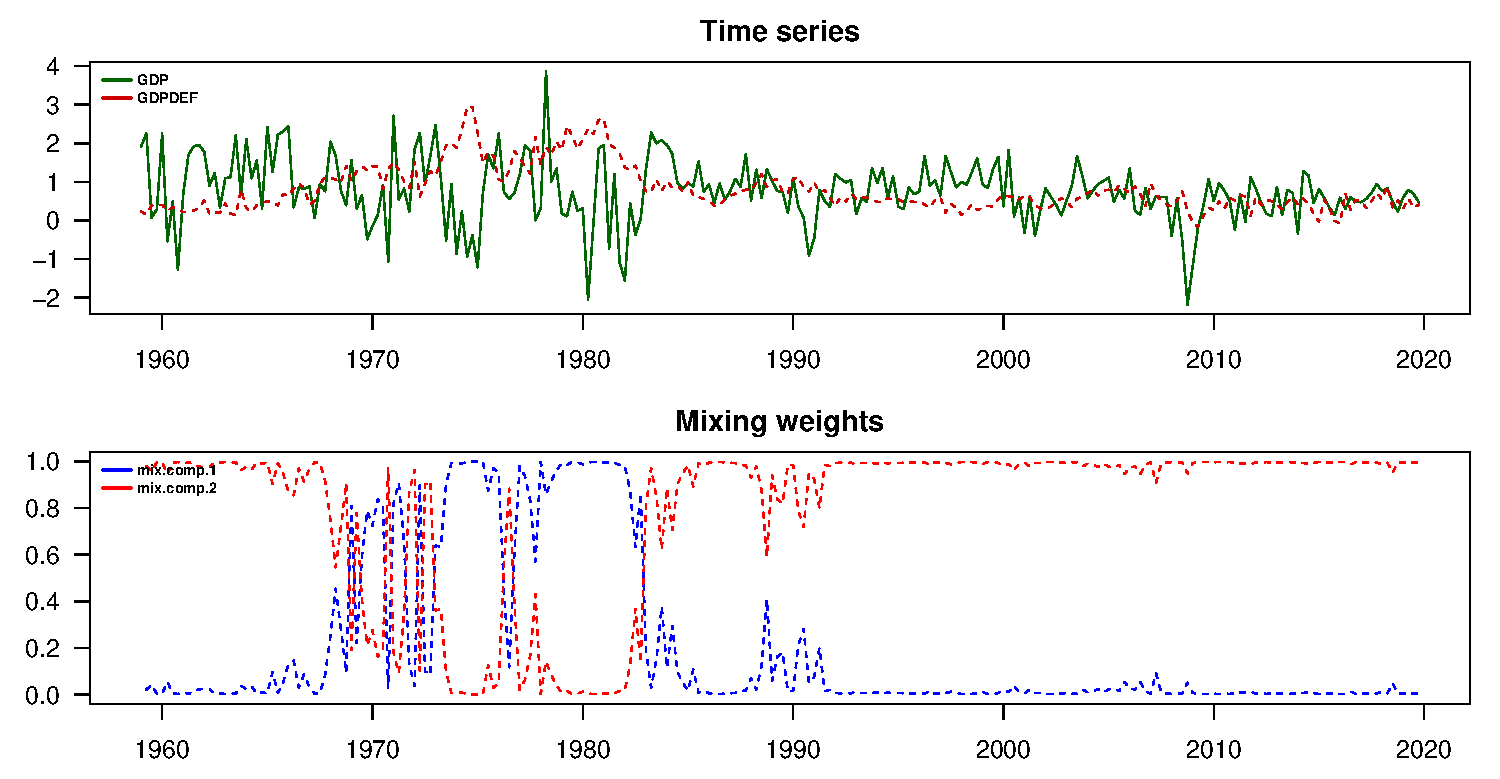
\includegraphics{gmvarkit-vignette-plotseries}
%

And the following command creates the stationary density plot:
%
\begin{Schunk}
\begin{Sinput}
R> plot(fit12gs, type="density")
\end{Sinput}
\end{Schunk}
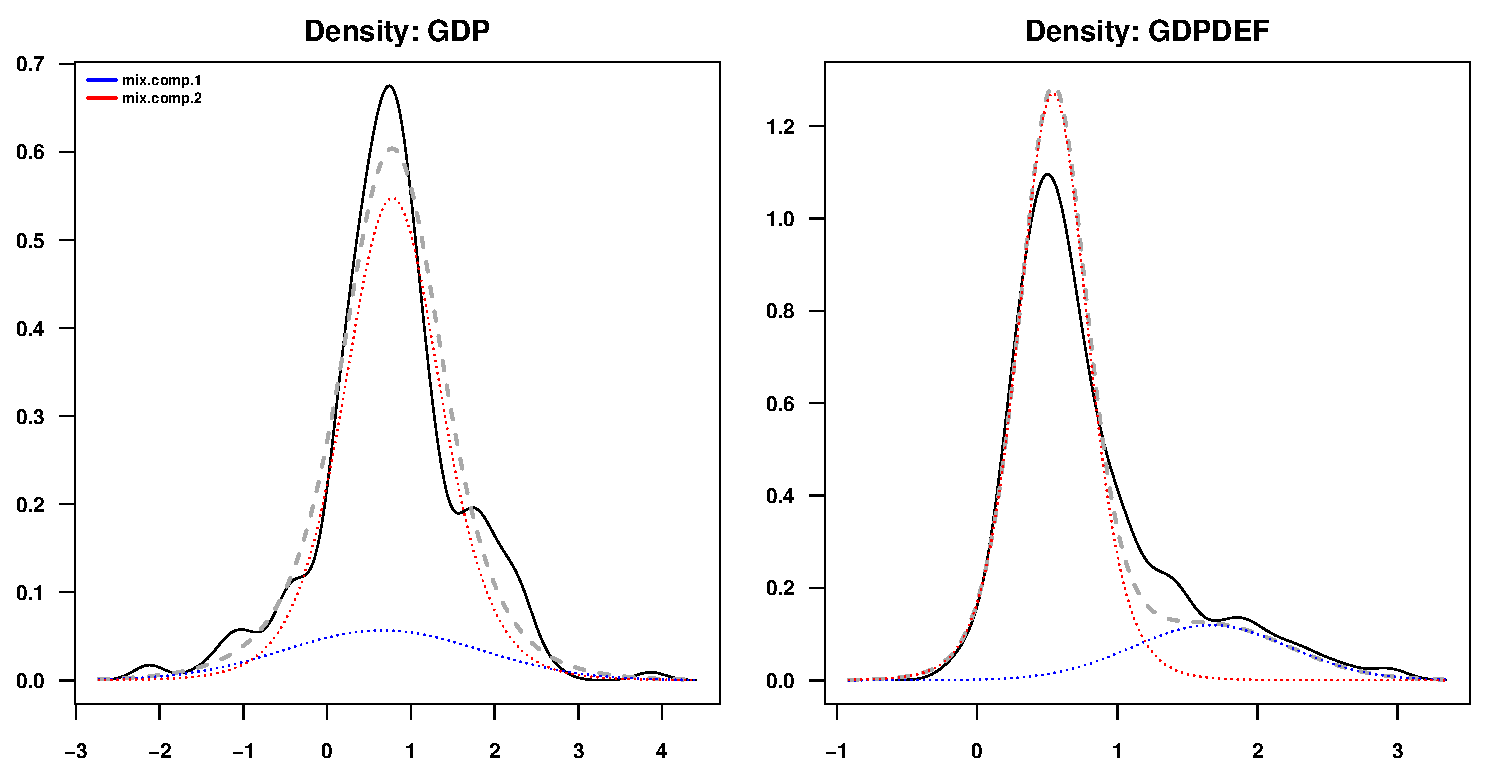
\includegraphics{gmvarkit-vignette-plotdensity}
%

If the argument \code{type} is not specified, both of the figures will be plotted.

It is also sometimes interesting to examine the time series of (one-step) conditional means and variances of the process along with the time series the model was fitted to. This can be done conveniently with the function \code{cond_moment_plot}, where the argument \code{which_moment} should be specified with \code{"mean"} or \code{"variance"} accordingly. In addition to the conditional moment of the process, \code{cond_moment_plot} also displays the conditional means or variances of the regimes multiplied by the mixing weights. Note, however, that the conditional variance of the process is not generally the same as the weighted sum of regimewise conditional variances, as it includes a component that encapsulates heteroskedasticity caused by variation in the conditional mean.


The variable metric algorithm employed in the final estimation does not necessarily stop at a local maximum point. The algorithm might also stop at a saddle point or near a local maximum, when the algorithm is not able to increase the log-likelihood, or at any point, when the maximum number of iterations has been reached. In the latter case, the estimation function throws a warning, but saddle points and inaccurate estimates need to be detected by the researcher.

It is well known that in a local maximum point, the gradient of the log-likelihood function is zero, and the eigenvalues of the Hessian matrix are all negative. In a local minimum, the eigenvalues of the Hessian matrix are all positive, whereas in a saddle point, some of them are positive and some negative. Nearly numerically singular Hessian matrices occur when the surface of the log-likelihood function is very flat about the estimate in some directions. This particularly happens when the model contains overly large degrees of freedom parameter estimates or the mixing weights $\alpha_{m,t}$ are estimated close to zero for all $t=1,...,T$ for some regime $m$.

\pkg{gmvarkit} provides several functions for evaluating whether the estimate is a local maximum point. The function \code{get_foc} returns the (numerically approximated) gradient of the log-likelihood function evaluated at the estimate, and the function \code{get_soc} returns eigenvalues of the (numerically approximated) Hessian matrix of the log-likelihood function evaluated at the estimate. The numerical derivatives are calculated using a central difference approximation
\begin{equation}
\frac{\partial L(\boldsymbol{\theta})}{\partial \theta_i} \approx \frac{f(\boldsymbol{\theta} + \boldsymbol{h}^{(i)}) - f(\boldsymbol{\theta} - \boldsymbol{h}^{(i)})}{2h}, \ \ h>0,
\end{equation}
where $\theta_i$ is the $i$th element of $\boldsymbol{\theta}$ and $\boldsymbol{h}^{(i)}=(0,...,0,h,0,...,0)$
contains $h$ as its $i$th element. By default, the difference $h=6\cdot 10^{-6}$ is used for all parameters except for overly large degrees of freedom parameters, whose partial derivatives are approximated using larger differences. The difference is increased for large degrees of freedom parameters, because the limited precision of the float point presentation induces artificially rugged surfaces to the their profile log-likelihood functions, and the increased differences diminish the related numerical error. On the other hand, as the surface of the profile log-likelihood function is very flat about a large degrees of freedom parameter estimate, large differences work well for the approximation.

For example, the following code calculates the first order condition for the G-StMVAR model \code{fit12gs}:
%
\begin{Schunk}
\begin{Sinput}
R> get_foc(fit12gs)
\end{Sinput}
\begin{Soutput}
 [1] -0.0006134447  0.0137299025  0.0098887109 -0.0011046216
 [5] -0.0082410002  0.0043358573  0.0227806301  0.0567827575
 [9] -0.0305398871 -0.0076389005  0.0217023555  0.0085821531
[13]  0.0139181727 -0.0017298992  0.0010732843  0.0213273026
[17]  0.0066026165 -0.2656223946  0.0142493946  0.0003786577
\end{Soutput}
\end{Schunk}
%
and the following code calculates the second order condition:
%
\begin{Schunk}
\begin{Sinput}
R> get_soc(fit12gs)
\end{Sinput}
\begin{Soutput}
 [1]     -0.129339     -1.391451    -12.777210    -18.688706
 [5]    -20.669182    -50.434083    -81.137635   -107.036071
 [9]   -171.759280   -212.430510   -277.544528   -337.194107
[13]   -446.790867  -1103.841017  -1130.123478  -1260.969931
[17]  -1821.309543  -9262.322334 -13026.702437 -34549.413869
\end{Soutput}
\end{Schunk}
%
All eigenvalues of the Hessian matrix are negative, which points to a local maximum, but the gradient of the log-likelihood function seems to somewhat deviate from zero. The gradient might be inaccurate, because it is based on a numerical approximation. It is also possible that the estimate is inaccurate, because it is based on approximative numerical estimation, and the estimates are therefore not expected to be exactly accurate. Whether the estimate is a local maximum point with accuracy that is reasonable enough, can be evaluated by plotting the graphs of the profile log-likelihood functions about the estimate. In \pkg{gmvarkit}, this can be done conveniently with the function \code{profile_logliks}.

The exemplify, the following command plots the graphs of profile log-likelihood functions of the estimated G-StMVAR model \code{fit12gs}:
%
\begin{Schunk}
\begin{Sinput}
R> profile_logliks(fit12gs, scale=0.02, precision=50)
\end{Sinput}
\end{Schunk}
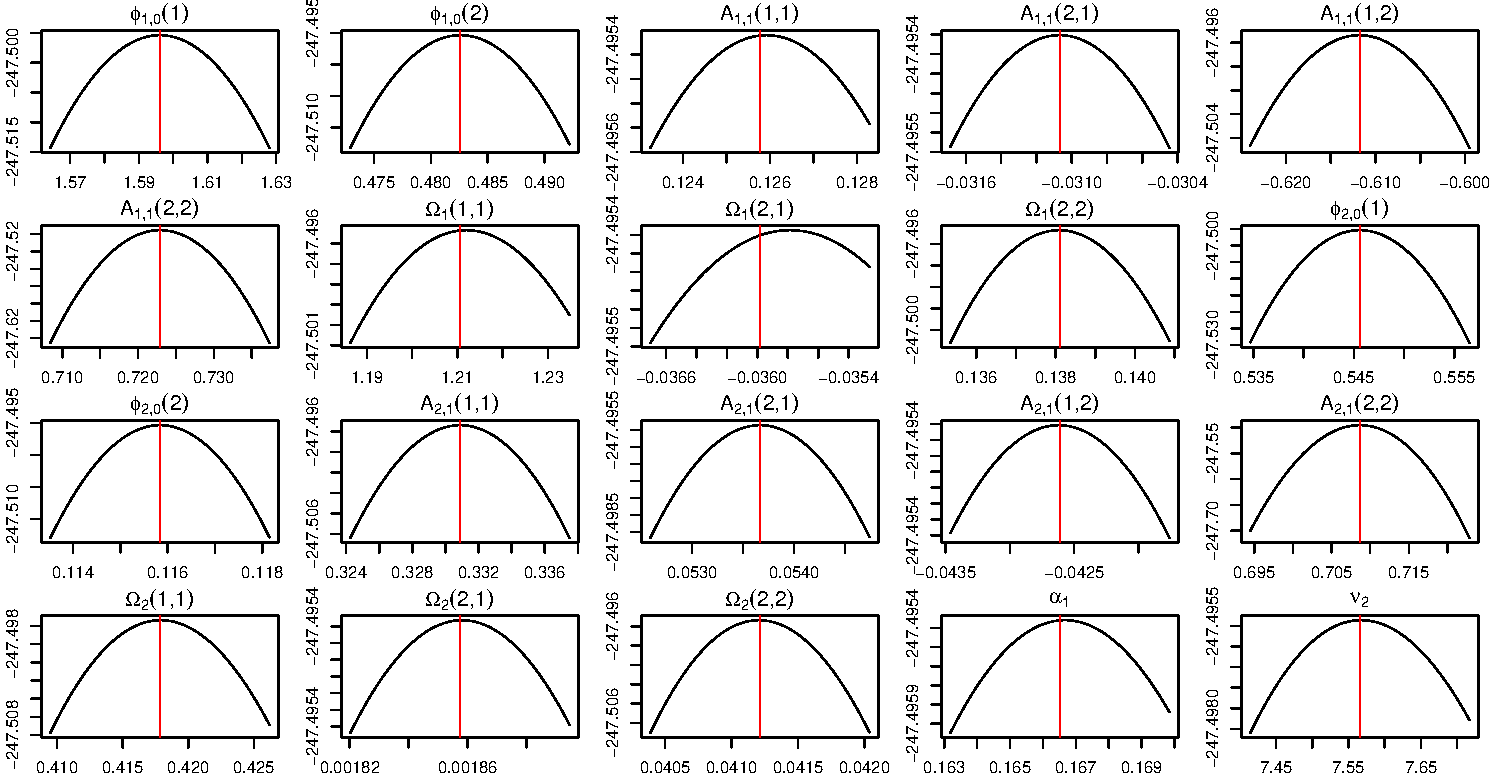
\includegraphics{gmvarkit-vignette-profilelogliks}
%

The output shows that the estimate's accuracy is reasonable, as changing any individual parameter value marginally would not increase the log-likelihood much. The argument \code{scale} can be adjusted to shorten or lengthen the interval shown in the horizontal axis. If one zooms in enough by setting \code{scale} to a very small number, it can be seen that the estimate is not exactly at the local maximum, but it is so close that moving there would not increase the log-likelihood notably. The argument \code{precision} can be adjusted to increase the number of points the graph is based on. For faster plotting, it can be decreased, and for more precision, it can be increased. The argument \code{which_pars} is used to specify the parameters whose profile log-likelihood functions should be plotted. This argument is particularly useful when creating as many plots as there are parameters in the model to a single figure would cause the individual plots to be very small. In such a case, profile log-likelihood functions for subsets of the parameters can be plotted separately by specifying this argument accordingly.

We have discussed tools that can be utilized to evaluate whether the found estimate is a local maximum with a reasonable accuracy. It is, however, more difficult to establish that the estimate is the global maximum. With \pkg{gmvarkit}, the best way to increase the reliability that the found estimate is the global maximum, is to run more estimation rounds by adjusting the argument \code{ncalls} of the estimation function \code{fitGSMVAR}. If the model is very large, a very large number of estimation rounds may be required to find the global maximum. If there are two regimes in the model, $p$ is reasonable, and the dimension of the time series at most four, the required number of estimation rounds typically varies from several hundred to several thousand depending on the model and the data. In the simpler models, less estimation rounds are required. In the larger models, and in particular if $M>2$, a significantly large number of estimation rounds may be required obtain the MLE.

\subsection{Estimation of the structural GSMVAR model}\label{sec:estim_structural}
The structural GSMVAR models are estimated similarly to the reduced form version, expect that the model is parametrized with $W$ and $\lambda_{mi}$, $m=2,...,M$, $i=1,...,d$ instead of the covariance matrices $\Omega_{m}$, $m=1,...,M$. The estimation is can be done with the function \code{fitGSMVAR} but now the argument \code{structural_pars} needs to be supplied with a list providing the constraints on $W$ (which equally imposes the constraints on the B-matrix) and optionally linear constraints on the $\lambda_{mi}$ parameters.

The list \code{structural_pars} should contain at least the element \code{W} which is a $(dxd)$ matrix matrix with its entries imposing constraints on $W$: \code{NA} indicating that the element is unconstrained, a positive value indicating strict positive sign constraint, a negative value indicating strict negative sign constraint, and zero indicating that the element is constrained to zero. The element named \code{C_lambda} is optional. If specified it should be a $(d(M-1) \times r)$ constraint matrix that satisfies ($\lambda_{2},...,\lambda_{M}) =C_{\lambda} \gamma$ where $\lambda_{m}=(\lambda_{m1},...,\lambda_{md})$ and $\gamma$ is the new $(r x 1)$ parameter subject to which the model is estimated (similarly to AR parameter constraints). The entries of \code{C_lambda} must be either positive or zero. Ignore (or set to \code{NULL}) if the eigenvalues $\lambda_{mi}$ should not be constrained. Note that other constraints than constraining some of the $\lambda_{mi}$ to be identical are not recommended but if such constraints are imposed, the argument \code{lambda_scale} in the genetic algorithm (see \code{?GAfit}) should be adjusted accordingly.

\textbf{Reliable estimation of structural GSMVAR models typically requires much more estimation rounds than the estimation of the reduced form models. However, when $M=2$, every reduced form model has an implied statistically identified structural model, which can be built without any additional estimation (see the next subsection). We recommend considering this implied model first. Then, if overidentifying constraints are to be imposed on the B-matrix (or equally $W$), we recommend using the unrestricted estimate to create an initial guess for the constrained parameter vector and pass this to the genetic algorithm as an initial population}. See the help page \code{?GAfit} for the arguments that can be passed by \code{fitGSMVAR} to the genetic algorithm. Create the initial guess for the parameter vector by using the form given in documentation of the argument \code{initpop}. If $M\neq 2$, the structural model needs to be estimated in the normal way with \code{fitGSMVAR}, however.

\subsubsection{Building structural model based on a reduced form model}
If the number of regimes is two ($M=2$), a structural model can be built based on a reduced form model, because the matrix decomposition used in the simultaneous diagonalization of the error term covariance matrices always exists. This can be done with function \code{gsmvar_to_sgsmvar} which should be supplied with the reduced form model, and it then returns a corresponding structural model. After creating the structural model, the columns of $W$ can be reordered with the function \code{reorder_W_columns} which also reorders all $\lambda_{mi}$ accordingly (and hence the resulting model will coincide with the original reduced form model). Also, all signs any column of $W$ can be swapped with the function \code{swap_W_signs} (and structural model is still related to the same reduced form model).

The exemplify, the following code creates statistically identified structural model based on the reduced form model \code{fit12gs} and then prints the estimates.
%
\begin{Schunk}
\begin{Sinput}
R> fit12gss <- gsmvar_to_sgsmvar(fit12gs)
R> fit12gss
\end{Sinput}
\begin{Soutput}
Structural G-StMVAR model:
 p = 1, M1 = 1, M2 = 1, d = 2, #parameters = 20, #observations = 244 x 2,
 conditional log-likelihood, intercept parametrization, no AR parameter constraints 

Regime 1 (GMVAR type)
Mixing weight: 0.17 
Regime means: 0.66, 1.67

   Y     phi0          A1                  Omega         1/2     
1 y1 = [ 1.60 ] + [  0.13 -0.61 ] y1.1 + [  1.21 -0.04 ]     eps1
2 y2   [ 0.48 ]   [ -0.03  0.72 ] y2.1   [ -0.04  0.14 ]     eps2

Regime 2 (StMVAR type)
Mixing weight: 0.83 
Regime means: 0.78, 0.54
Df parameter:  7.57

   Y     phi0          A1                            Omega         
1 y1 = [ 0.55 ] + [  0.33 -0.04 ] y1.1 + (         [  0.42 0.00 ] )
2 y2   [ 0.12 ]   [  0.05  0.71 ] y2.1   ( ARCH_mt [  0.00 0.04 ] )
  1/2     
1     eps1
2     eps2

Structural parameters:
        W             lamb2  
1 [  0.95 -0.55 ]   [  0.37 ]
2 [  0.16  0.34 ] , [  0.28 ]

The B-matrix (or equally W) is subject to 0 zero constraints and 2 sign constraints.
The eigenvalues lambda_{mi} are not subject to linear constraints.
\end{Soutput}
\end{Schunk}
%

Estimates for the structural parameters, $W$ and the eigenvalues, are printed last.

\subsection{Constrained estimation}\label{sec:examp_const}

\subsubsection{Imposing linear constraints and parameter vector}
Imposing linear constraints on the autoregressive parameters of GMVAR model is straightforward in \pkg{gmvarkit}. The constraints are expressed in a somewhat general form which allows to impose a wide class of constraints but one needs to take the time to construct the constraint matrix carefully for each particular case.

We consider constraints of form
\begin{align}
& (\boldsymbol{\phi}_1,...,\boldsymbol{\phi}_M) = \boldsymbol{C}\boldsymbol{\psi},\\
& \boldsymbol{\phi}_m=(vec(A_{m,1}),...,vec(A_{m,p}))\enspace (pd^2x1), \enspace m=1,...,M,
\end{align}
$\boldsymbol{C}$ is known $(Mpd^2xq)$ constraint matrix (of full column rank) and $\boldsymbol{\psi}$ is unknown $(qx1)$ parameter vector.

The parameter vector for constrained model has the size $((M(d+d(d+1)/2+1)+q-1)x1)$ and the form
\begin{equation}
\boldsymbol{\theta} = (\phi_{1,0},...,\phi_{M,0},\boldsymbol{\psi},\alpha_1,...,\alpha_{M-1}),
\end{equation}
where $\boldsymbol{\psi}$ is the $(qx1)$ parameter vector containing constrained autoregressive parameters. As in the case of regular models, instead of the intercept parametrization that takes use of intercept terms $\phi_{m,0}$, one may use the mean parametrization with regimewise means $\mu_m$ instead $(m=1,...,M)$.

\subsubsection{Examples of linear constraints}
Consider the following two common uses of linear constraints: restricting the autoregressive matrices to be the same for all regimes and constraining some AR parameters to zero. Of course also some other constraints may be useful, but we chose to show illustrative examples of these two, as they are taken use of in \cite{Kalliovirta+Meitz+Saikkonen:2016}.

\subsubsection{Restricting AR matrices to be the same for all regimes}
To restrict the AR matrices to be the same for all regimes, we want $\boldsymbol{\phi}_m$ to be the same for all $m=1,...,M$. The parameter vector $\boldsymbol{\psi}$ $(qx1)$ then corresponds to any $\boldsymbol{\phi}_m=\boldsymbol{\phi}$, and therefore $q=pd^2$. For the constraint matrix we choose
\begin{equation}
\boldsymbol{C} = [I_{pd^2}:\cdots:I_{pd^2}]' \enspace (Mpd^2xpd^2),
\end{equation}
that is, $M$ pieces of $(pd^2xpd^2)$ diagonal matrices stacked on top of each other, because then
\begin{equation}
\boldsymbol{C}\boldsymbol{\psi}=(\boldsymbol{\psi},...,\boldsymbol{\psi})=(\boldsymbol{\phi},...,\boldsymbol{\phi}).
\end{equation}
For instance, if there are two regimes in the model, the appropriate constraint matrix then created with \proglang{R} as
%
\begin{Schunk}
\begin{Sinput}
R> p <- 1 # Any autoregressive order
R> d <- 2 # Whatever the dimension of the time series is
R> I_pd2 <- diag(p*d^2) # The appropriate diagonal matrix
R> (C1 <- rbind(I_pd2, I_pd2)) # Stack them on top of each other
\end{Sinput}
\begin{Soutput}
     [,1] [,2] [,3] [,4]
[1,]    1    0    0    0
[2,]    0    1    0    0
[3,]    0    0    1    0
[4,]    0    0    0    1
[5,]    1    0    0    0
[6,]    0    1    0    0
[7,]    0    0    1    0
[8,]    0    0    0    1
\end{Soutput}
\end{Schunk}
%
The command \code{fitGSMVAR(gdpdef, p=1, M=2, model="GMVAR", constraints=C1)} would then estimate a GMVAR($1,2$) model with the AR matrices constrained to be the same in both regimes. In practice, you might want to adjust the number of estimation rounds and set seeds. Notably, with the dimension of the time series being only two and $p=1$ with two regimes, almost all of the estimation rounds end up in the MLE. Also, because model has the AR matrices constrained to be the same for all regimes, the estimation is much easier than with freely estimated models.

\subsubsection{Restricting AR parameters to be the same for all regimes and constraining non-diagonal elements of coefficient matrices to be zero}
The previous example shows how to restrict the AR parameters to be the same for all regimes, but say we also want to constrain the non-diagonal elements of coefficient matrices $A_{m,i}$ $(m=1,...,M, i=1,...,p)$ to be zero. We have the constrained parameter $\boldsymbol{\psi}$ $(qx1)$ representing the unconstrained parameters $(\boldsymbol{\phi_1},...,\boldsymbol{\phi}_M)$, where by assumption $\boldsymbol{\phi}_m=\boldsymbol{\phi}=(vec(A_1),...,vec(A_p))$ $(pd^2x1)$ and the elements of $vec(A_i)$ $(i=1,...,p)$ corresponding to the diagonal are zero.

For illustrative purposes, let's consider a GMVAR model with autoregressive degree $p=2$, number of mixture components $M=2$ and number of time series in the system $d=2$. Then we have
\begin{align}
\boldsymbol{\phi}&=(A_1(1,1),0,0,A_1(2,2),A_2(1,1),0,0,A_2(2,2)) \enspace (8x1) \enspace \text{and}
\boldsymbol{\psi}&=(A_1(1,1),A_1(2,2),A_2(1,1),A_2(2,2)) \enspace (4x1).
\end{align}
By a direct calculation, we can see that choosing the constraint matrix
\begin{equation}
\boldsymbol{C}=\left[{\begin{array}{c}
   \boldsymbol{\tilde{c}} \\
   \boldsymbol{\tilde{c}} \\
  \end{array}}\right]
\enspace (Mpd^2x4),
\enspace
\end{equation}
where
\begin{equation}
\boldsymbol{\tilde{c}}=\left[{\begin{array}{cccc}
   1 & 0 & 0 & 0 \\
   0 & 0 & 0 & 0 \\
   0 & 0 & 0 & 0 \\
   0 & 1 & 0 & 0 \\
   0 & 0 & 1 & 0 \\
   0 & 0 & 0 & 0 \\
   0 & 0 & 0 & 0 \\
   0 & 0 & 0 & 1 \\
  \end{array}}\right]
\enspace (pd^2x4)
\end{equation}
satisfies $\boldsymbol{C}\boldsymbol{\psi}=(\boldsymbol{\phi},...,\boldsymbol{\phi}).$

The above constraint matrix can be created with \proglang{R} as
%
\begin{Schunk}
\begin{Sinput}
R> c_tilde <- matrix(0, nrow=2*2^2, ncol=4)
R> c_tilde[c(1, 12, 21, 32)] <- 1
R> c_tilde
\end{Sinput}
\begin{Soutput}
     [,1] [,2] [,3] [,4]
[1,]    1    0    0    0
[2,]    0    0    0    0
[3,]    0    0    0    0
[4,]    0    1    0    0
[5,]    0    0    1    0
[6,]    0    0    0    0
[7,]    0    0    0    0
[8,]    0    0    0    1
\end{Soutput}
\begin{Sinput}
R> C2 <- rbind(c_tilde, c_tilde)
\end{Sinput}
\end{Schunk}
%
The command \code{fitGSMVAR(gdpdef, p=2, M=2, model="GMVAR", constraints=C2)} would then estimate a GMVAR($2,2$) model with the AR matrices constrained to be the same in both regimes and the off-diagonal elements constrained to zero (again, you may want to adjust the argument \code{ncalls}).

\subsubsection{Constraining the unconditional means of some regimes to be the same}
In addition to constraining the autoregressive parameters, \pkg{gmvarkit} allows to constrain the unconditional means of some regimes to be the same. This feature is, however, only available for models that are parametrized with the unconditional means instead of intercepts (because some of the estimation is always done with mean-parametrization and one cannot generally swap the parametrization when constraints are imposed on means/intercepts). With the mean-parametrization employed (by setting \code{parametrization="mean"}), one may define groups of regimes that have the same mean parameters using the argument \code{same_means}. For instance, with three regime model $(M=3)$ the argument \code{same_means=list(c(1, 3), 2)} sets the unconditional means of the first and third regimes to be the same while allows the second regime to have different mean.

One can also combine linear constraints on the AR parameters with constraining some of the means to be the same. This allows, for instance, to estimate a model in which only the covariance matrix varies in time. Validity of different constraints can be evaluated, for example, with likelihood ratio and Wald tests using the functions \code{LR_test} and \code{Wald_test}.

To exemplify, the following code (which is not executed in this vignette) estimates a GMVAR($p=4, M=2$) model such that the unconditional means and autoregression matrices are constrained be the same in both regimes. The resulting model thereby has time-varying covariance matrix but otherwise it is linear.
%
\begin{CodeChunk}
\begin{CodeInput}
R> I_pd2 <- diag(4*2^2) # The appropriate diagonal matrix for the constraint matrix
R> C3 <- rbind(I_pd2, I_pd2) # Stack them on top of each other
R> fit42cm <- fitGSMVAR(gdpdef, p=4, M=2, model="GMVAR", parametrization="mean",
+               same_means=list(1:2), constraints=C3, ncalls=20, seeds=1:20)
\end{CodeInput}
\end{CodeChunk}
%


\subsection{Testing parameter constraints}\label{sec:testconst}
One way to asses the validity of the imposed constraints is to compare the values of information criteria of the constrained and unconstrained models. \pkg{gmvarkit}, however, also provides functions for testing the constraints with the likelihood ratio test and Wald test, which are applicable as the ML estimator of a GSMVAR model has the conventional asymptotic distribution \cite[as long as the model is correctly specified and one is willing to assume the validity of the required unverified assumptions; see][Theorem 3, and \cite{Kalliovirta+Meitz+Saikkonen:2016}, Theorem 3]{Virolainen2:2021}. For a discussion on the likelihood ratio and Wald tests, see \citet{Buse:1982} and the references therein, for example.

The likelihood ratio test considers the null hypothesis that the true parameter value $\boldsymbol{\theta}_0$ satisfies some constraints imposed on these parameters \cite[such that the constrained parameter space is a subset of the parameter space, which is presented in][Assumption 2 for the GSMVAR models]{Virolainen2:2021}. Denoting by $\hat{L}_U$ and $\hat{L}_C$ the (maximized) log-likelihoods based on the unconstrained and constrained ML estimates, respectively, the test statistic takes the form
\begin{equation}
LR=2(\hat{L}_U - \hat{L}_C).
\end{equation}
Under the null, the test statistic is asymptotically $\chi^2$-distributed with the degrees of freedom given by the difference in the dimensions of the unconstrained and constrained parameter spaces. With \pkg{gmvarkit}, the likelihood ratio test can be calculated with the function \code{LR_test}, which takes the unconstrained model (a class \code{gsmvar} object) as its first argument and the constrained model as the second argument.

\pkg{gmvarkit} implements the Wald test of the null hypothesis
\begin{equation}
A\boldsymbol{\theta}_0 = c,
\end{equation}
where $A$ is a $(k \times d)$ matrix with full row rank, $c$ is a $(k \times 1)$ vector, $\boldsymbol{\theta}_0$ is the true parameter value, $d$ is the dimension of the parameter space, and $k$ is the number of constraints. The Wald test statistic takes the form
\begin{equation}
W = (A\hat{\boldsymbol{\theta}} - c)' [A\mathcal{J}(\hat{\boldsymbol{\theta}})^{-1}A']^{-1}(A\hat{\boldsymbol{\theta}} - c),
\end{equation}
where $\mathcal{J}(\hat{\boldsymbol{\theta}})$ is the observed information matrix evaluated at the ML estimate $\hat{\boldsymbol{\theta}}$. Under the null, the test statistic is asymptotically $\chi^2$-distributed with $k$ degrees of freedom (which is the difference in dimensions of the constrained and unconstrained parameter spaces). With \pkg{gmvarkit}, the Wald test can be calculated with function \code{Wald_test}, which takes the estimated unconstrained model (as a class \code{gsmvar} object) as the first argument, the matrix $A$ as the second argument, and the vector $c$ as the third argument.

Note that the standard tests are not applicable if the number of GMVAR or StMVAR type regimes is chosen too large, as then some of the parameters are not identified, causing the result of the asymptotic normality of the ML estimator to break down. This particularly happens when one tests for the number of regimes in the model, as the under the null some of the regimes are reduced from the model\footnote{\cite{Meitz+Saikkonen:2021} have, however, recently developed such tests for mixture models with Gaussian conditional densities} \citep[see the related discussion in][]{Virolainen2:2021}. Similar caution applies for testing whether a regime is of the GMVAR type against the alternative that it is of the StMVAR type: then $\nu_m = \infty$ under the null for the regime $m$ to be tested, which violates the assumption that the parameter value is in the interior of a compact subset of the parameter space \citep[see][Theorem 3 and Assumption 1]{Virolainen2:2021}.


\section{Quantile residual based model diagnostics}\label{sec:qres}
In the GSMVAR models, the empirical counterparts of the error terms $\varepsilon_{m,t}$ in (\ref{eq:defeq}) cannot be calculated, because the regime that generated each observation is unknown, making the conventional residual based diagnostics unavailable. Therefore, \pkg{gmvarkit} utilizes so called \emph{quantile residuals}, which are suitable for evaluating adequacy of the GSMAR models.

Denote by $y_t$, $t=1,2,...$,  the time series of interest and $\mathcal{F}_{t-1}$ the $\sigma$-algebra generated by the random variables or vectors $\lbrace y_{t-j}, j > 0 \rbrace$.  Moreover, let $\boldsymbol{\theta}$ denote the relevant parameter vector. \cite{Kalliovirta:2012} defines univariate quantile residuals as
\begin{equation}
R_{t,\boldsymbol{\theta}}=\Phi^{-1}(F(y_t;\boldsymbol{\theta}\mid \mathcal{F}_{t-1})),
\end{equation}
where $\Phi(\cdot)^{-1}$ is the standard normal quantile function and $F(\cdot\mid \mathcal{F}_{t-1})$ is the conditional distribution function of the considered model.

\cite{Kalliovirta+Saikkonen:2010} define multivariate quantile residuals analogously to the univariate ones but by taking into account the dependence of the component time series from each other.  Denote $\mathcal{A}_{j-1}=\sigma(y_{1,t},...,y_{j-1,t})$ and by $f(\cdot|\sigma(\mathcal{F}_{t-1},\mathcal{A}_{j-1}))=f_{j-1,t-1}(\cdot)$ the conditional density function conditional on the $\sigma$-algebra $\sigma(\mathcal{F}_{t-1},\mathcal{A}_{j-1})$

The conditional density function of the random vector $y_t$ can be expressed in a product form by conditioning to the components $y_t$ in addition to the history $\mathcal{F}_{t-1}$ as
\begin{equation}\label{eq:prodform}
f(y_t;\theta|\mathcal{F}_{t-1})=\prod_{j=1}^{d}f_{j-1,t-1}(y_{j,t};\boldsymbol{\theta}),
\end{equation}
where $y_{j,t}$ is the $j$th component of $y_t$ and $f_{0,t-1}(y_{1,t};\boldsymbol{\theta})=f_{1,t-1}(y_{1,t};\boldsymbol{\theta})$ is the marginal conditional density function of $y_{1,t}$ conditional on $\mathcal{F}_{t-1}$.

The conditional distribution functions corresponding to the density functions $f_{j-1,t-1}(\cdot;\boldsymbol{\theta})$ in (\ref{eq:prodform}) are of the form
\begin{equation}
F_{j-1,t-1}(y_{j,t};\boldsymbol{\theta})=\int_{-\infty}^{y_{j,t}} f_{j-1,t-1}(u;\boldsymbol{\theta})du.
\end{equation}

The multivariate quantile residuals are then defined as
\begin{equation}\label{eq:qrdef}
R_{t,\boldsymbol{\theta}}=
\begin{bmatrix}
  R_{1t,\boldsymbol{\theta}} \\
  R_{2t,\boldsymbol{\theta}} \\
  \vdots \\
  R_{dt,\boldsymbol{\theta}} \\
\end{bmatrix} =
\begin{bmatrix}
  \Phi^{-1}(F_{0,t-1}(y_{1,t};\boldsymbol{\theta})) \\
  \Phi^{-1}(F_{1,t-1}(y_{2,t};\boldsymbol{\theta}))\\
  \vdots \\
  \Phi^{-1}(F_{d-1,t-1}(y_{d,t};\boldsymbol{\theta})) \\
\end{bmatrix},
\end{equation}
and its empirical counterpart, $r_{t,\hat{\boldsymbol{\theta}}}$,  is obtained by replacing the parameter $\boldsymbol{\theta}$ with its maximum likelihood (ML) estimate $\hat{\boldsymbol{\theta}}$. Closed form expressions for the quantile residuals of the G-StMVAR model (which encompasses GMVAR and StMVAR models as special cases) are derived in Appendix~\ref{ap:qresexpr}

For a correctly specified GSMVAR model employing the ML estimator, the empirical counterparts of multivariate quantile residuals are asymptotically multivariate standard normal \citep[Lemma 3]{Kalliovirta+Saikkonen:2010}. They can therefore be utilized in graphical diagnostic simalarly to the conventional Pearson's residuals. For the graphical diagnostics, \pkg{gmvarkit} provides function \code{diagnostic_plot} which plots the quantile residual time series, auto- and crosscorrelations of the quantile residuals, auto- and crosscorrelations of the squared quantile residuals, and normal quantile-quantile plots as well as histrograms of the quantile residuals.

\cite{Kalliovirta+Saikkonen:2010} also propose three diagnostic tests for testing normality, autocorrelation, and conditional heteroskedasticity of the quantile residuals. The tests can be based either on the data or on a simulation procedure. If the sample is short, tests based on the data can be too forgiving, so to obtain more reliable test results the simulation procedure is recommended (with sample size of at least several thousand). The tests can be calculated with \pkg{gmvarkit} by using the function \code{quantile_residual_tests}. The simulation procedure is employed if the argument \code{nsim} is set larger the number of observations (in each component time series). In this case, \code{nsim} sets the length of the sample path used in the simulation procedure.




\section{Impulse response analysis}\label{sec:impulseresponse}

\subsection{Generalized impulse response function}
We consider the generalized impulse response function (GIRF) \cite{Koop+Pesaran+Potter:1996} defined as
\begin{equation}\label{eq:girf}
\text{GIRF}(n,\delta_j,\mathcal{F}_{t-1}) = \text{E}[y_{t+n}|\delta_j,\mathcal{F}_{t-1}] - \text{E}[y_{t+n}|\mathcal{F}_{t-1}],
\end{equation}
where $n$ is the chosen horizon, $\mathcal{F}_{t-1}=\sigma\lbrace y_{t-j},j>0\rbrace$ as before, the first term in the RHS is the expected realization of the process at time $t+n$ conditionally on a structural shock of magnitude $\delta_j \in\mathbb{R}$ in the $j$th element of $e_t$ at time $t$ and the previous observations, and the second term in the RHS is the expected realization of the process conditionally on the previous observations only. GIRF thus expresses the expected difference in the future outcomes when the specific structural shock hits the system at time $t$ as opposed to all shocks being random.

Due to the $p$-step Markov property of the SG-StMVAR model, conditioning on (the $\sigma$-algebra generated by) the $p$ previous observations $\boldsymbol{y}_{t-1}\equiv(y_{t-1},...,y_{t-p})$ is effectively the same as conditioning on $\mathcal{F}_{t-1}$ at the time $t$ and later. The history $\boldsymbol{y}_{t-1}$ can be either fixed or random, but with random history the GIRF becomes a random vector, however. Using fixed $\boldsymbol{y}_{t-1}$ makes sense when one is interested in the effects of the shock in a particular point of time, whereas more general results are obtained by assuming that $\boldsymbol{y}_{t-1}$ follows the stationary distribution of the process. If one is, on the other hand, concerned about a specific regime, $\boldsymbol{y}_{t-1}$ can be assumed to follow the stationary distribution of the corresponding component model.

In practice, the GIRF and its distributional properties can be approximated with a Monte Carlo algorithm that generates independent realizations of the process and then takes the sample mean for point estimate. If $\boldsymbol{y}_{t-1}$ is random and follows the distribution $G$, the GIRF should be estimated for different values of $\boldsymbol{y}_{t-1}$ generated from $G$, and then the sample mean and sample quantiles can be taken to obtain the point estimate and confidence intervals. The algorithm implemented in `gmvarkit` is presented in an Appendix of \cite{Virolainen:2020}.

Because the SG-StMVAR model allows to associate specific features or economic interpretations for different regimes, it might be interesting to also examine the effects of a structural shock to the mixing weights $\alpha_{m,t}$, $m=1,...,M$. We then consider the related GIRFs $E[\alpha_{m,t+n}|\delta_j,\boldsymbol{y}_{t-1}] - E[\alpha_{m,t+n}|\boldsymbol{y}_{t-1}]$ for which point estimates and confidence intervals can be constructed similarly to (\ref{eq:girf}).

In \pkg{gmvarkit}, the GIRF can be estimated with the function \code{GIRF} which should be supplied with the estimated SG-StMVAR model or a SG-StMVAR model build with hand specified parameter values using the function \code{GMVAR}. The size of the structural shock can be set with the argument \code{shock_size}. If not specified, the size of one standard deviation is used; that is, the size one. Among other arguments, the function may also be supplied with the argument \code{init_regimes} which specifies from which regimes' stationary distributions the initial values are generated from. If more than one regime is specified, a mixture distribution with weights given by the mixing weight parameters is used. Alternatively, one may specify fixed initial values with the argument \code{init_values}. Note that the confidence intervals (whose confidence level can be specified with the argument \code{ci}) reflect uncertainty about the initial value only and not about the parameter estimates.

Because estimating the GIRF and confidence intervals for it is computationally demanding, parallel computing is taken use of to shorten the estimation time. The number of CPU cores used can be set with the argument \code{ncores}. The objects returned by the \code{GIRF} function have their own \code{plot} and \code{print} methods. Also, cumulative impulse responses of the specified variables can be obtained directly by specifying the argument \code{which_cumulative}, while scaled GIRFs can be obtained by specifying the argument \code{scale} as desired.

\subsection{Generalized forecast error variance decomposition}
We consider the generalized forecast error variance decomposition (GFEVD) \cite{Lanne+Nyberg:2016}  that is defined for variable $i$, shock $j$, and horizon $n$ as
\begin{equation}
\text{GFEVD}(n,y_{it}, \delta_j,\mathcal{F}_{t-1}) = \frac{\sum_{l=0}^n\text{GIRF}(l,\delta_j,\mathcal{F}_{t-1})_i^2}{\sum_{k=1}^d\sum_{l=0}^n\text{GIRF}(l,\delta_k,\mathcal{F}_{t-1})_i^2},
\end{equation}
where $n$ is the chosen and $\text{GIRF}(l,\delta_j,\mathcal{F}_{t-1})_i$ is the $i$th element of the related GIRF (see also the notation described for GIRF in the previous section). That is, the GFEVD is otherwise similar to the conventional forecast error variance decomposition but with GIRFs in the place of conventional impulse response functions. Because the GFEVDs sum to unity (for each variable), they can be interpreted in a similar manner to the conventional FEVD.

In \pkg{gmvarkit}, the GFEVD can be estimated with the function \code{GFEVD}. As with the GIRF, the GFEVD is dependent on the initial values. The type of the initial values is set with the argument \code{initval_type}, and there are three options:
\begin{enumerate}
\item \code{"data"} which estimates the GIRFs for all possible length $p$ histories in the data and then the GIRFs in the GFEVD are obtained as the sample mean over those GIRFs.
\item \code{"random"} which generates the initial values from the stationary distribution of the process or from the mixture of the stationary distributions of some specific regime(s) with the relative mixing proportions given by the mixing weight parameters. The initial regimes can be set with the argument \code{init_regimes}. The GIRFs in the GFEVD are obtained as the sample mean over the GIRFs estimated for the different random initial values.
\item \code{"fixed"} which estimates the GIRFs for a single fixed initial value that is set with the argument \code{init_ values}.
\end{enumerate}
The shock size is the same for all scalar components of the structural shock and it can be adjusted with the argument \code{shock_size}. If the GIRFs for some variables should be cumulative before calculating the GFEVD, specify them with the argument \code{which_cumulative}. Finally, note that the GFEVD objects have their own plot and print methods.



\section{Building a GSMVAR model with specific parameter values}\label{sec:GSMVAR}
The function \code{GSMVAR} facilitates building GSMVAR models without estimation, for instance, in order to simulate observations from a GSMVAR process with specific parameter values. The parameter vector (of length $M(d + d^2p + d(d+1)/2 + 2) - M_1 - 1$ for unconstrained reduced form models) has the form $\boldsymbol{\theta} = (\boldsymbol{\vartheta}_1,...,\boldsymbol{\vartheta}_M,\alpha_1,...,\alpha_{M-1},\boldsymbol{\nu})$ where
\begin{align}
\boldsymbol{\vartheta}_m &= (\varphi_{m,0},\text{vec}({A_{m,1}}),...,\text{vec}(A_{m,p}),\text{vech}(\Omega_m),\ \ m=1,...,M, \ \text{and}  \\
\boldsymbol{\nu} &= (\nu_{M_1+1},...,\nu_M).
\end{align}
%
In the GMVAR model (when $M_1=M$), the vector $\boldsymbol{\nu}$ is omitted, as the GMVAR model does not contain degrees of freedom parameters. For models with constraints on the autoregressive parameters, the parameter vectors are expressed in a different way. They are only presented in the package documentation for brevity, because the hand-specified parameter values can be set to satisfy any constraints as is. In a structural GSMVAR model, the parameter vector has the form
\begin{align}
\boldsymbol{\theta} &= (\varphi_{1,0},...,\varphi_{M,0},\text{vec}(\boldsymbol{A}_1),...,\text{vec}(\boldsymbol{A}_M),\text{vec}(W),\boldsymbol{\lambda}_1,...,\boldsymbol{\lambda}_M, \alpha_1,...,\alpha_{M-1},\boldsymbol{\nu}), \\
\boldsymbol{A}_m & = (\text{vec}({A_{m,1}}),...,\text{vec}(A_{m,p})) \\
\boldsymbol{\lambda}_m &= (\lambda_{m1},...,\boldsymbol{\lambda}_{md}).
\end{align}
For constrained structural models (including constraints on the structural parameters), see the documentation of \code{GSMVAR} (or any other relevant function).

In addition to the parameter vector, \code{GSMVAR} should be supplied with arguments \code{p} and \code{M} specifying the order of the model similarly to the estimation function \code{fitGSMVAR} discussed in Sections \ref{sec:example_estim}. If one wishes to parametrize the model with the regimewise unconditional means ($\mu_m$) instead of the intercepts ($\varphi_{m,0}$), the argument \code{parametrization} should be set to \code{"mean"} in which case the intercept parameters $\varphi_{m,0}$ are replaced with $\mu_m$ in the parameter vector. By default, \pkg{gmvarkit} uses intercept parametrization.

To exemplify, we build a reduced form StMVAR $p=1$, $M=1$, $d=2$ model. The model has intercept parametrization and parameter values $\varphi_{1,0}=(0, 1)$ $\text{vec}(A_{1,1}) = (0.2, 0.2, 0.2, -0.2)$, $\vech{\Omega}_2 = (1, 0.1, 1)$, and $\nu_1 = 3$. After building the model, we use the \code{print} method to examine it:
%
\begin{Schunk}
\begin{Sinput}
R> params112 <- c(0, 1, 0.2, 0.2, 0.2, -0.2, 1, 0.1, 1, 3)
R> mod112 <- GSMVAR(p=1, M=1, d=2, params=params112, model="StMVAR")
R> mod112
\end{Sinput}
\begin{Soutput}
Reduced form StMVAR model:
 p = 1, M = 1, d = 2, #parameters = 10, 
 conditional log-likelihood, intercept parametrization, no AR parameter constraints 

Regime 1
Mixing weight: 1.00 
Regime means: 0.22, 0.87
Df parameter:  3.00

   Y     phi0          A1                            Omega         
1 y1 = [ 0.00 ] + [  0.20  0.20 ] y1.1 + (         [  1.00 0.10 ] )
2 y2   [ 1.00 ]   [  0.20 -0.20 ] y2.1   ( ARCH_mt [  0.10 1.00 ] )
  1/2     
1     eps1
2     eps2
\end{Soutput}
\end{Schunk}
%

It is possible to include data in the models built with \code{GSMVAR} by either providing the data in the argument \code{data} when creating the model or by adding the data afterwards with the function \code{add_data}. When the model is supplied with data, the mixing weights, one-step conditional means and variances, and quantile residuals can be calculated and included in the model. The function \code{add_data} can also be used to update data to an estimated GSMVAR model without re-estimating the model.


\section{Simulation and forecasting}\label{sec:simufore}

\subsection{Simulation}\label{sec:simu}
\pkg{gmvarkit} implements the S3 method \code{simulate} for simulating observations from GSMVAR processes (see \code{?simulate.gsmvar}). The method requires the process to be given as a class \code{gsmvar} object, which are typically created either by estimating a model with the function \code{fitGSMVAR} or by specifying the parameter values by hand and building the model with the constructor function \code{GSMVAR}. The initial values required to simulate the first $p$ observations can be either set by hand (with the argument \code{init_values}) or drawn from the stationary distribution of the process (by default) or from a (mixture of) stationary distribution(s) of given regime(s). The argument \code{nsim} sets the length of the sample path to be simulated.

To give an example, the following code sets the random number generator seed to one and simulates 500 observations long sample from the StMVAR process built in Section~\ref{sec:GSMVAR}:
%
\begin{CodeChunk}
\begin{CodeInput}
R> mysim <- simulate(mod112, nsim=500, seed=1)
\end{CodeInput}
\end{CodeChunk}
%
Our implementation of \code{simulate} returns a list containing the simulated sample path in \code{$sample}, the mixture component that generated each observation in \code{$component}, and the mixing weights in \code{$mixing_weights}.

\subsection{Simulation based forecasting}
Deriving multiple-steps-ahead point predictions and prediction intervals analytically for the GSMVAR models is very complicated, so \pkg{gmvarkit} employs the following simulation-based method. By using the last $p$ observations of the data up to the date of forecasting as initial values, a large number of sample paths for the future values of the process are simulated. Then, sample quantiles from the simulated sample paths are calculated to obtain prediction intervals, and the median or mean is used for point predictions. A similar procedure is also applied to forecast future values of the mixing weights, which might be of interest because the researcher can often associate specific characteristics to different regimes.

Forecasting is most conveniently done with the \code{predict} method (see \code{?predict.gsmvar}). The available arguments include the number of steps ahead to be predicted (\code{n_ahead}), the number sample paths the forecast is based on (\code{nsim}), possibly multiple confidence levels for prediction intervals (\code{pi}), prediction type (\code{pred_type}), and prediction interval type (\code{pi_type}). The prediction type can be either \code{median}, \code{mean}, or for one-step-ahead forecasts also the exact conditional mean, \code{cond_mean}. The prediction interval type can be any of \code{"two-sided"}, \code{"upper"}, \code{"lower"}, or \code{"none"}.

To exemplify, the following code forecasts the two-dimensional time-series of U.S. GDP and GDP deflator growth using the G-StMVAR($1, 1, 1$) model \code{fit12gs} estimated in Section~\ref{example_est}. The forecast is $10$ steps (quarters in this case) ahead, based on $100$ Monte Carlo repetitions with the point forecast based on the mean of those repetitions. The prediction intervals are two-sided with confidence levels $0.95$ and $0.90$. Finally, the argument \code{mix_weights} states that also future values of the the mixing weights should be forecasted. After completing the forecast, the function plots the results by default.
%
\begin{Schunk}
\begin{Sinput}
R> mypred <- predict(fit12gs, n_ahead=10, nsim=100, pred_type="mean",
+                    pi_type="two-sided", pi=c(0.95, 0.90),
+                    mix_weights=TRUE)
\end{Sinput}
\end{Schunk}
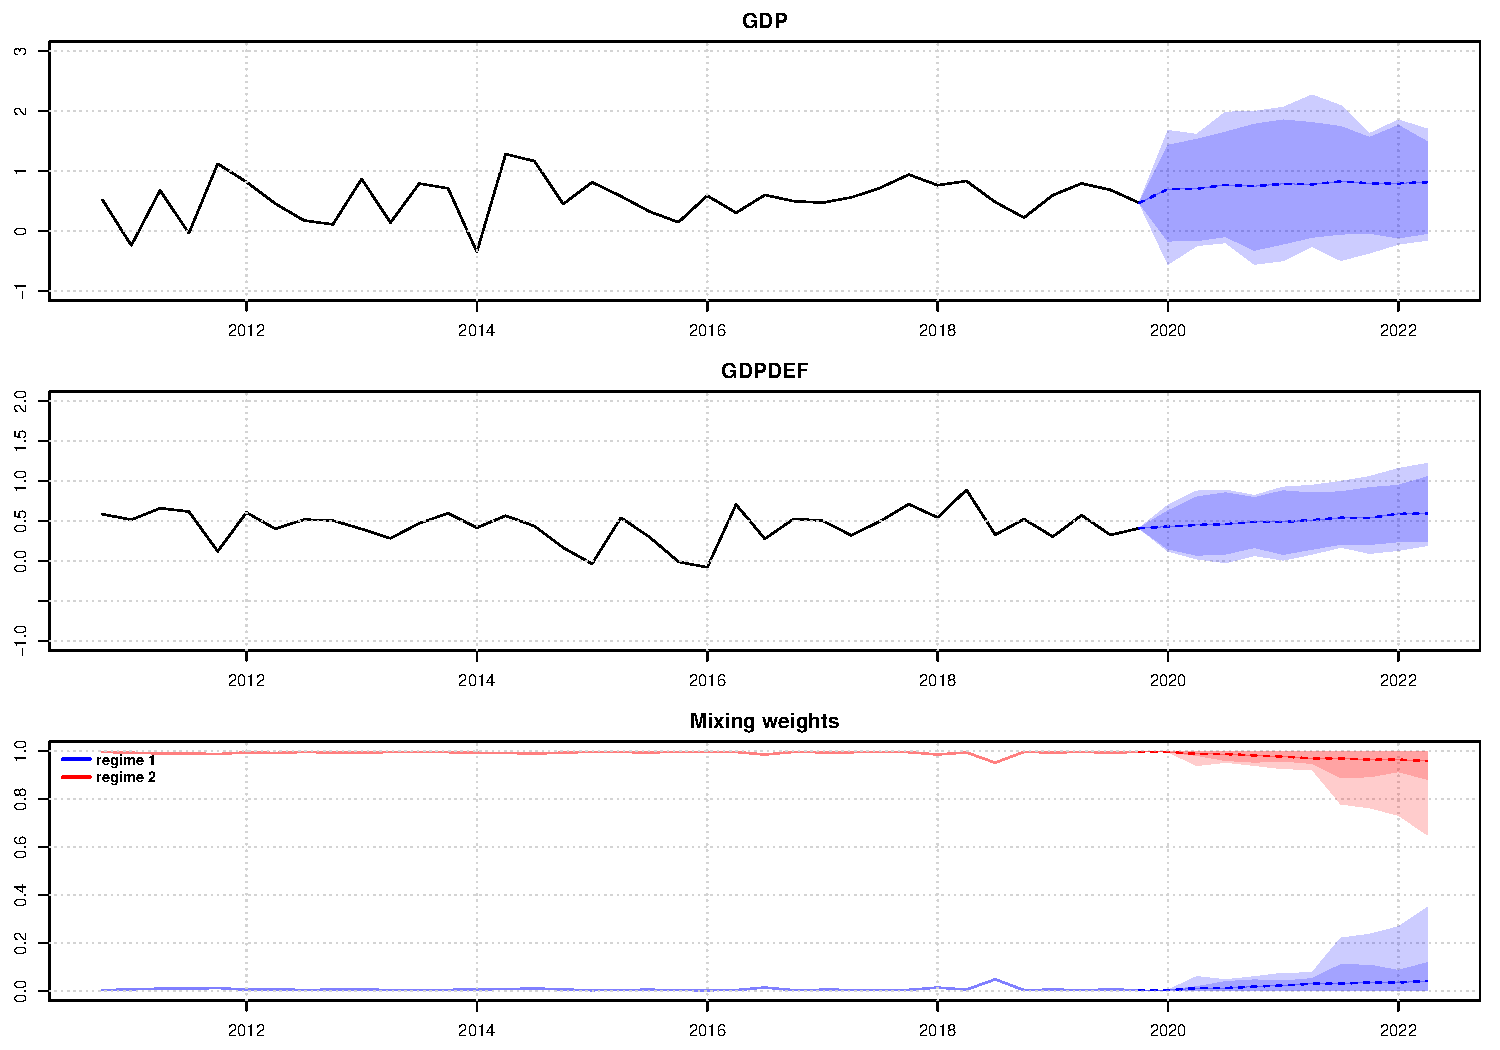
\includegraphics{gmvarkit-vignette-predict}
%





\begin{table}
\centering
\begin{tabular}{llp{6.4cm}}
\hline
Related to     & Name                      & Description \\ \hline
Estimation     & \code{fitGSMVAR}           & Estimate a GSMVAR model.\\
               & \code{alt_gsmvar}          & Build a GSMVAR model based on results from any estimation round.\\
               & \code{stmvar_to_gstmvar}    & Estimate a G-StMVAR model based on a StMVAR (or G-StMVAR) model with large degrees of freedom parameters.\\
               & \code{iterate_more}       & Run more iterations of the variable metric algorithm for a preliminary estimated GSMVAR model.\\
Estimates      & \code{summary} (method)   & Detailed printout of the estimates.\\
               & \code{plot} (method)      & Plot the series with the estimated mixing weights and a kernel density estimates of the (marginal) series with the (marginal) stationary densities of the model.\\
               & \code{get_foc}            & Calculate numerically approximated gradient of the log-likelihood function evaluated at the estimate.\\
               & \code{get_soc}            & Calculate eigenvalues of numerically approximated Hessian of the log-likelihood function evaluated at the estimate.\\
               & \code{profile_logliks}    & Plot the graphs of the profile log-likelihood functions.\\
               & \code{cond_moment_plot}   & Plot the model implied one-step conditional means or variances.\\
Diagnostics    & \code{quantile_residual_tests} & Calculate quantile residual tests.\\
               & \code{diagnostic_plot}    & Plot quantile residual diagnostics.\\
Forecasting    & \code{predict} (method)   & Forecast future observations and mixing weights of the process.\\
Simulation     & \code{simulate} (method)  & Simulate from a GSMVAR process.\\
Create model   & \code{GSMVAR}              & Construct a GSMVAR model based on specific parameter values.\\
Hypothesis testing & \code{LR_test}        & Calculate likelihood ratio test.\\
               & \code{Wald_test}          & Calculate Wald test.\\
Other          & \code{add_data}           & Add data to a GSMVAR model \\
               & \code{swap_parametrization} & Swap between mean and intercept parametrizations \\
\hline
\end{tabular}
\caption{Some useful functions in \pkg{gmvarkit} sorted according to their usage. The note "method" in parentheses after the name of a function signifies that it is an S3 method for a class \code{gsmvar} object (often generated by the function \code{fitGSMVAR} or \code{GSMVAR}).}
\label{tab:functions}
\end{table}

\section{Summary}\label{sec:summary}
Mixture vector autoregressive models are a valuable tool in modeling multivariate time series in which the data generating dynamics vary in time. We described the \proglang{R} package \pkg{gmvarkit}, which accommodates the GMVAR model \citep{Kalliovirta+Meitz+Saikkonen:2016}, the StMVAR model \citep{Virolainen2:2021}, and the G-StMVAR model \citep{Virolainen2:2021} - an appealing family of mixture autoregressive models that call the GSMVAR models. We discussed several features provided by \pkg{gmvarkit} for GSMVAR modeling: unconstrained and constrained maximum likelihood estimation of the model parameter, hypothesis testing, quantile residual based model diagnostics, estimation of generalized impulse response function and generalized forecast error variance decomposition, simulation, forecasting, and more. For convenience, we have collected some useful function in \pkg{gmvarkit} to Table~\ref{tab:functions}.


\pagebreak
\bibliography{refs}

\newpage

\begin{appendix}
\section{Properties of multivariate Gaussian and Student's $t$ distribution}\label{ap:propt}
Denote a $d$-dimensional real valued vector by $y$.  It is well known that the density function of a $d$-dimensional Gaussian distribution with mean $\mu$ and covariance matrix $\Sigma$ is
\begin{equation}
n_d(y;\mu,\Sigma) = (2\pi)^{-d/2}\text{det}(\Sigma)^{-1/2}\exp\left\lbrace -\frac{1}{2}(y -\mu)'\Sigma^{-1}(y - \mu) \right\rbrace .
\end{equation}
Similarly to \cite{Meitz+Preve+Saikkonen:2021} but differing from the standard form, we parametrize the Student's $t$-distribution using its covariance matrix as a parameter together with the mean and the degrees of freedom. The density function of such a $d$-dimensional $t$-distribution with mean $\mu$, covariance matrix $\Sigma$, and $\nu>2$ degrees of freedom is
\begin{equation}
t_d(y;\mu,\Sigma,\nu)=C_d(\nu)\text{det}(\Sigma)^{-1/2}\left(1+\frac{(y -\mu)'\Sigma^{-1}(y - \mu)}{\nu-2}\right)^{-(d+\nu)/2},
\end{equation}
where
\begin{equation}
C_d(\nu)=\frac{\Gamma\left(\frac{d+\nu}{2}\right)}{\sqrt{\pi^d(\nu-2)^d}\Gamma\left(\frac{\nu}{2}\right)},
\end{equation}
and $\Gamma\left(\cdot\right)$ is the gamma function.  We assume that the covariance matrix $\Sigma$ is positive definite for both distributions.

Consider a partition $X=(X_1,X_2)$ of either Gaussian or $t$-distributed (with $\nu$ degrees of freedom) random vector $X$ such that $X_1$ has dimension $(d_1\times1)$ and $X_2$ has dimension $(d_2\times1)$. Consider also a corresponding partition of the mean vector $\mu=(\mu_1,\mu_2)$ and the covariance matrix
\begin{equation}
\Sigma=
\begin{bmatrix}
\Sigma_{11} & \Sigma_{12} \\
\Sigma_{12}' & \Sigma_{22}
\end{bmatrix},
\end{equation}
where, for example, the dimension of $\Sigma_{11}$ is $(d_1\times d_1)$.  In the Gaussian case, $X_1$ then has the marginal distribution $n_{d_1}(\mu_1,\Sigma_{11})$ and $X_2$ has the marginal distribution $n_{d_2}(\mu_2,\Sigma_{22})$.  In the Student's $t$ case,  $X_1$ has the marginal distribution $t_{d_1}(\mu_1,\Sigma_{11},\nu)$ and $X_2$ has the marginal distribution $t_{d_2}(\mu_2,\Sigma_{22},\nu)$ (see, e.g., \cite{Ding:2016}, also in what follows).

When $X$ has Gaussian distribution,  the conditional distribution of the random vector $X_1$ given $X_2=x_2$ is
\begin{equation}
X_1\mid(X_2=x_2)\sim n_{d_1}(\mu_{1\mid2}(x_2),\Sigma_{1\mid2}(x_2)),
\end{equation}
where
\begin{align}
\mu (x_2)\equiv \mu_{1\mid2}(x_2) &= \mu_1+\Sigma_{12}\Sigma_{22}^{-1}(x_2-\mu_2) \quad \text{and}\label{eq:mux_gaus} \\
\Omega \equiv \Sigma_{1\mid2}(x_2) &= \Sigma_{11}-\Sigma_{12}\Sigma_{22}^{-1}\Sigma_{12}'. \label{eq:omegax_gaus}
\end{align}

When $X$ has $t$-distribution, the conditional distribution of the random vector $X_1$ given $X_2=x_2$ is
\begin{equation}
X_1\mid(X_2=x_2)\sim t_{d_1}(\mu_{1\mid2}(x_2),\Sigma_{1\mid2}(x_2),\nu+d_2),
\end{equation}
where
\begin{align}
\mu (x_2) = \mu_{1\mid2}(x_2) &= \mu_1+\Sigma_{12}\Sigma_{22}^{-1}(x_2-\mu_2) \quad \text{and}\label{eq:mux} \\
\Omega (x_2) \equiv \Sigma_{1\mid2}(x_2) &= \frac{\nu-2+(x_2-\mu_2)'\Sigma_{22}^{-1}(x_2-\mu_2)}{\nu-2+d_2}(\Sigma_{11}-\Sigma_{12}\Sigma_{22}^{-1}\Sigma_{12}'). \label{eq:omegax}
\end{align}
In particular, we have
\begin{align}\label{eq:td_decomp}
n_d(x;\mu,\Sigma) &= n_{d_1}(x_1;\mu_{1|2}(x_2),\Sigma_{1|2}(x_2))t_{d_2}(x_2;\mu_2,\Sigma_{22}) \quad \text{and}\\
t_d(x;\mu,\Sigma,\nu) &= t_{d_1}(x_1;\mu_{1|2}(x_2),\Sigma_{1|2}(x_2),\nu+d_2)t_{d_2}(x_2;\mu_2,\Sigma_{22},\nu).
\end{align}



\section{Quantile residuals of the G-StMVAR model}\label{ap:qresexpr}
The conditional density function of the $d$-dimensional G-StMVAR process $y_t$ conditional on  $\mathcal{F}_{t-1}$ is
\begin{equation}\label{eq:gstmvarconddens}
f_{t-1}(y_t;\boldsymbol{\theta})=\sum_{m=1}^{M_1}\alpha_{m,t}n_d(y_t;\mu_{m,t},\Omega_{m}) + \sum_{m=M_1+1}^{M}\alpha_{m,t}t_d(y_t;\mu_{m,t},\Omega_{m,t},\nu_m + dp),
\end{equation}
where $n_d(\cdot;\mu_{m,t},\Omega_m,\nu_m + dp)$ is the density function of $d$-dimensional normal distribution with mean $\mu_{m,t}$ and covariance matrix $\Omega_{m}$; and  $t_d(\cdot;\mu_{m,t},\Omega_m,\nu_m + dp)$ is the density function of $d$-dimensional $t$-distribution with mean $\mu_{m,t}$, covariance matrix $\Omega_{m,t}$,  and $\nu_m + dp$ degrees of freedom.

Denote $y_t^{(k)}=(y_{1,t},...,y_{k,t})$ $(k\times 1)$,  $k\leq d$,   $\mu_{m,t}^{(k)}=(\mu_{1,m,,t},...,\mu_{k,m,t})$ $(k\times 1)$,  $k\leq d$,  and by $\Omega_{m,t}^{(k)}$ ($\Omega_{m}^{(k)}$) the upper left $(k\times k)$ block matrix of $\Omega_{m,t}$ ($\Omega_{m}$).  Then,  the properties of the marginal distributions of multivariate Gaussian and $t$-distributions (see Appendix~\ref{ap:propt}) show that conditional on $\mathcal{F}_{t-1}$,  the random vectors $y_t^{(j)}$, $j=1,..,d$,  follow the distribution that is a mixture $M_1$ $j$-dimensional normal distributions (with means $\mu_{m,t}^{(j)}$ and covariance matrices $\Omega_{m}^{(j)}$) and $M_2\equiv M-M_1$ $j$-dimensional $t$-distributions (with means $\mu_{m,t}^{(j)}$,  covariance matrices $\Omega_{m,t}^{(j)}$, and $\nu_m + dp$ degrees of freedom).  The mixing weights $\alpha_{m,t}$ are not affected, as they are $\mathcal{F}_{t-1}$-measurable.  Therefore, the marginal density function of $y_t^{(j)}$ is
\begin{equation}\label{eq:ytj_margdens}
f_{t-1}(y_{t}^{(j)};\boldsymbol{\theta})=\sum_{m=1}^{M_1}\alpha_{m,t} n_j(y_{t}^{(j)};\mu_{m,t}^{(j)},\Omega_{m}^{(j)}) + \sum_{m=M_1 + 1}^{M}\alpha_{m,t} t_j(y_{t}^{(j)};\mu_{m,t}^{(j)},\Omega_{m,t}^{(j)},\nu_m + dp),
\end{equation}

The conditional density function $f_{0,t-1}(y_{1,t};\boldsymbol{\theta})$ in (\ref{eq:prodform}) is obtained from (\ref{eq:ytj_margdens}) by choosing $j=1$.  For $j=2,...,d$,  the conditional density functions  $f_{j-1,t-1}(y_{j,t};\boldsymbol{\theta})$ are obtained by substituting the equation (\ref{eq:ytj_margdens}) to the formula of conditional density function:
\begin{align}\label{eq:conddens_gstmvar}
\begin{aligned}
&f_{j-1,t-1}\left(y_{j,t};\boldsymbol{\theta}\right) = \frac{f_{t-1}(y_{t}^{(j)};\boldsymbol{\theta})}{f_{t-1}(y_{t}^{(j-1)};\boldsymbol{\theta})} = \\
&\frac{\sum_{m=1}^{M_1}\alpha_{m,t} n_j(y_{t}^{(j)};\mu_{m,t}^{(j)},\Omega_{m}^{(j)}) + \sum_{m=M_1+1}^{M}\alpha_{m,t} t_j(y_{t}^{(j)};\mu_{m,t}^{(j)},\Omega_{m,t}^{(j)}, \nu_m+dp)}{\sum_{n=1}^{M_1}\alpha_{n,t} n_{j-1}(y_{t}^{(j-1)};\mu_{n,t}^{(j-1)},\Omega_n^{(j-1)}) + \sum_{n=M_1+1}^{M}\alpha_{n,t} t_{j-1}(y_{t}^{(j-1)};\mu_{n,t}^{(j-1)},\Omega_n^{(j-1)},\nu_m + dp)}.
\end{aligned}
\end{align}

It follows from the properties of the conditional distributions of multivariate normal distribution that we may express the $j$-dimensional normal distributions as
\begin{equation}\label{eq:n1_nj-1}
n_j(y_{t}^{(j)};\mu_{m,t}^{(j)},\Omega_m^{(j)}) = n_1(y_{j,t};\mu_{m,t,j|j-1},\Omega_{m,j|j-1}) n_{j-1}(y_{t}^{(j-1)};\mu_{m,t}^{(j-1)},\Omega_m^{(j-1)}),
\end{equation}
where $\mu_{m,t,j|j-1}$ and $\Omega_{m,j|j-1}$ are the conditional mean and covariance matrix of $y_{j,t}$ conditional on $\sigma(\mathcal{A}_{j-1},\mathcal{F}_{t-1})$.  Likewise, it follows from the properties of the conditional distributions of multivariate $t$-distribution that we may express the $j$-dimensional $t$-distributions as
\begin{align}\label{eq:t1_tj-1}
\begin{aligned}
t_j(y_{t}^{(j)};\mu_{m,t}^{(j)},\Omega_{m,t}^{(j)},\nu_m + dp) =& t_1(y_{j,t};\mu_{m,t,j|j-1},\Omega_{m,t,j|j-1},\nu_m + dp + j  - 1) \\
&\times t_{j-1}(y_{t}^{(j-1)};\mu_{m,t}^{(j-1)},\Omega_{m,t}^{(j-1)},\nu_m + dp),
\end{aligned}
\end{align}
where $\mu_{m,t,j|j-1}$ and $\Omega_{m,t,j|j-1}$ are the conditional mean and covariance matrix of $y_{j,t}$ conditional on $\sigma(\mathcal{A}_{j-1},\mathcal{F}_{t-1})$.

By denoting
\begin{equation}\label{eq:beta_mtj_t}
\beta_{m,t,j} \equiv \frac{\alpha_{m,t}n_{j-1}(y_{t}^{(j-1)};\mu_{m,t}^{(j-1)},\Omega_{m}^{(j-1)})}{\sum_{n=1}^{M_1}\alpha_{n,t} n_{j-1}(y_{t}^{(j-1)};\mu_{n,t}^{(j-1)},\Omega_{n}^{(j-1)}) +\sum_{n=M_1+1}^{M}\alpha_{n,t} t_{j-1}(y_{t}^{(j-1)};\mu_{n,t}^{(j-1)},\Omega_{n,t}^{(j-1)},\nu_n + dp)}
\end{equation}
for $m=1,..,M_1$,  $j=2,...,d$,  and
\begin{equation}\label{eq:beta_mtj_t}
\beta_{m,t,j} \equiv \frac{\alpha_{m,t}t_{j-1}(y_{t}^{(j-1)};\mu_{m,t}^{(j-1)},\Omega_{m,t}^{(j-1)},\nu_m + dp)}{\sum_{n=1}^{M_1}\alpha_{n,t} n_{j-1}(y_{t}^{(j-1)};\mu_{n,t}^{(j-1)},\Omega_{n}^{(j-1)}) +\sum_{n=M_1+1}^{M}\alpha_{n,t} t_{j-1}(y_{t}^{(j-1)};\mu_{n,t}^{(j-1)},\Omega_{n,t}^{(j-1)},\nu_n + dp)}
\end{equation}
for $m=M_1+1,...,M$,  $j=2,...,d$, and using the expressions (\ref{eq:n1_nj-1}) and (\ref{eq:t1_tj-1}),  we can express the conditional density function (\ref{eq:conddens_gstmvar}) as
\begin{align}
\begin{aligned}
f_{j-1,t-1}\left(y_{j,t};\boldsymbol{\theta}\right)=&\sum_{m=1}^{M_1}\beta_{m,t,j}n_1(y_{j,t};\mu_{m,t,j|j-1},\Omega_{m,j|j-1})\\
& + \sum_{m=M_1+1}^{M}\beta_{m,t,j}t_1(y_{j,t};\mu_{m,t,j|j-1},\Omega_{m,t,j|j-1},\nu_m + dp + j - 1), \ \ j=2,..,d.
\end{aligned}
\end{align}

For $m=1,...,M_1$, the conditional means $\mu_{m,t,j|j-1}$ and covariance matrices $\Omega_{m,j|j-1}$ are as in (\ref{eq:mux_gaus}) and (\ref{eq:omegax_gaus}) when for each $j=2,...,d$ and $m=1,...,M$ we consider the partition $y_t^{(j)}=(y_t^{(j-1)},y_{j,t})$, $\mu_{m,t}^{(j)}=(\mu_{m,t}^{(j-1)},\mu_{j,m,t})$, and
\begin{equation}
\Omega_m^{(j)}=
\begin{bmatrix}
\Omega_m^{(j-1)} \quad\enspace & \Omega_{(j-1),j,m} \\
\Omega_{(j-1),j,m}' & \Omega_{m}(j,j)  \\
\end{bmatrix},
\end{equation}
where $\Omega_{m}(j,j)$ is the $jj$th elementh of $\Omega_m$ and $\Omega_{(j-1),j,m}$ $((j-1)\times 1)$  consists of the rows $1,...,j-1$ of the $j$th column of $\Omega_m$.  In particular, we have
\begin{align}
\mu_{m,t,j|j-1} &=\mu_{j,m,t} + \Omega_{(j-1),j,m}'(\Omega_m^{(j-1)})^{-1}(y_t^{(j-1)}-\mu_{m,t}^{(j-1)}),\label{eq:cond_mu_mtj_n}\\
\Omega_{m,j|j-1} &= \Omega_{m}(j,j) - \Omega_{(j-1),j,m}'(\Omega_m^{(j-1)})^{-1} \Omega_{(j-1),j,m}. \label{eq:cond_omega_mj_n}
\end{align}

For $m=M_1+1,..,M$, the conditional means $\mu_{m,t,j|j-1}$ and covariance matrices $\Omega_{m,t,j|j-1}$ are as in (\ref{eq:mux}) and (\ref{eq:omegax}) when for each $j=2,...,d$ and $m=1,...,M$ we consider the partition $y_t^{(j)}=(y_t^{(j-1)},y_{j,t})$, $\mu_{m,t}^{(j)}=(\mu_{m,t}^{(j-1)},\mu_{j,m,t})$, and
\begin{equation}
\Omega_{m,t}^{(j)}=
\begin{bmatrix}
\Omega_{m,t}^{(j-1)} \quad\enspace & \Omega_{(j-1),j,m,t} \\
\Omega_{(j-1),j,m,t}' & \Omega_{m,t}(j,j)  \\
\end{bmatrix},
\end{equation}
where $\Omega_{m,t}(j,j)$ is the $jj$th elementh of $\Omega_{m,t}$ and $\Omega_{(j-1),j,m,t}$ $((j-1)\times 1)$  consists of the rows $1,...,j-1$ of the $j$th column of $\Omega_{m,t}$.  In particular,  taking use of the relation $\Omega_{m,t}=\omega_{m,t}\Omega_m$ (where $\omega_{m,t}$ is scalar), we have
\begin{align}
\begin{aligned}
\mu_{m,t,j|j-1} &=\mu_{j,m,t} + \Omega_{(j-1),j,m,t}'(\Omega_{m,t}^{(j-1)})^{-1}(y_t^{(j-1)}-\mu_{m,t}^{(j-1)})\\
&=\mu_{j,m,t} + \Omega_{(j-1),j,m}'(\Omega_{m}^{(j-1)})^{-1}(y_t^{(j-1)}-\mu_{m,t}^{(j-1)}),
\end{aligned}\label{eq:cond_mu_mtj}
\end{align}
and
\begin{align}
\begin{aligned}
\Omega_{m,t,j|j-1} &= \frac{\nu_m + dp + (y_t^{(j-1)} - \mu_{m,t}^{(j - 1)})'(\Omega_{m,t}^{(j-1)})^{-1}(y_t^{(j-1)} - \mu_{m,t}^{(j - 1)})}{\nu_m + dp + j - 3}\tilde{\Omega}_{m,t,j|j-1}\\
&= \frac{\nu_m + dp + \omega_{m,t}^{-1}(y_t^{(j-1)} - \mu_{m,t}^{(j - 1)})'(\Omega_{m}^{(j-1)})^{-1}(y_t^{(j-1)} - \mu_{m,t}^{(j - 1)})}{\nu_m + dp + j - 3}\tilde{\Omega}_{m,t,j|j-1},
\end{aligned}\label{eq:cond_omega_mtj}
\end{align}
where
\begin{align}
\begin{aligned}
\tilde{\Omega}_{m,t,j|j-1} &\equiv \Omega_{m,t}(j,j) - \Omega_{(j-1),j,m,t}'(\Omega_{m,t}^{(j-1)})^{-1} \Omega_{(j-1),j,m,t}\\
&=\omega_{m,t}(\Omega_{m}(j,j) - \Omega_{(j-1),j,m}'(\Omega_{m}^{(j-1)})^{-1} \Omega_{(j-1),j,m}).
\end{aligned}
\end{align}

The conditional distribution functions $F_{i_j,j-1,t-1}(y_{i_j,t};\boldsymbol{\theta})$ in the definition of multivariate quantile residuals (\ref{eq:qrdef}) can be expressed as

It then remains to find expressions for the conditional distribution functions $F_{j-1,t-1}(y_{j,t};\boldsymbol{\theta})$, $j=1,...,d$, in (\ref{eq:qrdef}).  For notational convenience, we write
\begin{align}
\begin{aligned}
f_{j-1,t-1}(y_{j,t}\boldsymbol{\theta}) =& \sum_{m=1}^{M_1}\beta_{m,t,j}n_1(y_{j,t};\mu_{m,t,j|j-1},\Omega_{m,j|j-1}) \\
&+ \sum_{m=M_1 + 1}^{M}\beta_{m,t,j}t_1(y_{j,t};\mu_{m,t,j|j-1},\Omega_{m,t,j|j-1},\nu_m + dp + j - 1)
\end{aligned}
\end{align}
for all $j=1,...,d$ by defining $\beta_{m,t,1}\equiv \alpha_{m,t}$,  $\mu_{m,t,1|0}\equiv \mu_{m,t}^{(1)}$,  $\Omega_{m,1|0}\equiv \Omega_{m}^{(1)}$, and $\Omega_{m,t,1|0}\equiv \Omega_{m,t}^{(1)}$.  For $j=2,...,d$,  these quantities are defined in (\ref{eq:beta_mtj_t}), (\ref{eq:cond_mu_mtj_n}), (\ref{eq:cond_omega_mj_n}), (\ref{eq:cond_mu_mtj}), and (\ref{eq:cond_omega_mtj}). Then,
\begin{align}
\begin{aligned}
F_{j-1,t-1}(y_{j,t};\boldsymbol{\theta})=&\sum_{m=1}^{M_1}\beta_{m,t,j}\int_{-\infty}^{y_{j,t}}n_1(u;\mu_{m,t,j|j-1},\Omega_{m,j|j-1})du \\
&+\sum_{m=M_1+1}^{M}\beta_{m,t,j}\int_{-\infty}^{y_{j,t}}t_1(u;\mu_{m,t,j|j-1},\Omega_{m,t,j|j-1},\nu_m + dp + j - 1)du,
\end{aligned}
\end{align}
where we seek to solve the integrals inside the sums.

Regarding the first sum,  for $m=1,...,M_1$,  it is easy to see that the integrals can be expressed using the stardard normal distribution function $\Phi(\cdot)$ as
\begin{align}
\int_{-\infty}^{y_{j,t}}n_1(u;\mu_{m,t,j|j-1},\Omega_{m,j|j-1})du &= \Phi\left(\frac{y_{j,t}-\mu_{m,t,j|j-1}}{\sqrt{\Omega_{m,j|j-1}}}\right).
\end{align}

Next, consider the second sum,  $m=M_1+1,...,M$. By taking use of the symmetry of the $t$-distribution about its mean, we obtain
\begin{align}\label{eq:integral1}
\begin{aligned}
&\int_{-\infty}^{y_{j,t}}t_1(u;\mu_{m,t,j|j-1},\Omega_{m,t,j|j-1},\nu_m + dp + j - 1)du \\
&= \frac{1}{2} + \int_{\mu_{m,t,j|j-1}}^{y_{j,t}}t_1(u;\mu_{m,t,j|j-1},\Omega_{m,t,j|j-1},\nu_m + dp + j - 1)du.
\end{aligned}
\end{align}
By applying the change of variables $\tilde{u}_{m,t,j} = u - \mu_{m,t,j|j-1}$ in the integral, the RHS of (\ref{eq:integral1}) can be expressed as
\begin{equation}\label{eq:integral2}
\frac{1}{2} + \frac{\Gamma\left(\frac{\nu_m + dp + j}{2}\right)}{\sqrt{\pi (\nu_m + dp + j - 3)}\Gamma\left(\frac{\nu_m + dp + j - 1}{2} \right)}\Omega_{m,t,j|j-1}^{-1/2}\int_{0}^{\tilde{y}_{m,t,j}}\left(1 + \frac{\tilde{u}_{m,t,j}^2}{a_{m,t,j}} \right)^{-b_{m,j}}d\tilde{u}_{m,t,j},
\end{equation}
where $\tilde{y}_{m,t,j} \equiv y_{j,t} - \mu_{m,t,j|j-1}$,  $a_{m,t,j} \equiv (\nu_m + dp + j - 3)\Omega_{m,t,j|j-1}$, and $b_{m,j}\equiv (\nu_m + dp + j)/2$.

Then, by applying the change of variables $z_{m,t,j} =  \tilde{u}_{m,t,j}^2/\tilde{y}_{m,t,j}$,  we can express the integral in (\ref{eq:integral2}) as
\begin{equation}\label{eq:integral3}
\int_{0}^{\tilde{y}_{m,t,j}}\left(1 + \frac{\tilde{u}_{m,t,j}^2}{a_{m,t,j}} \right)^{-b_{m,j}}d\tilde{u}_{m,t,j} = \frac{1}{2}\int_{0}^{\tilde{y}_{m,t,j}}\left(\frac{\tilde{y}_{m,t,j}}{z_{m,t,j}}  \right)^{1/2}\left(1 + \frac{z_{m,t,j}\tilde{y}_{m,t,j}}{a_{m,t,j}} \right)^{-b_{m,j}}dz_{m,t,j}.
\end{equation}
By applying the third change of variables $x_{m,t,j}=z_{m,t,j}/\tilde{y}_{m,t,j}$ and using the properties of the gamma function,  the RHS of (\ref{eq:integral3}) can be expressed as
\begin{equation}
\frac{\tilde{y}_{m,t,j}}{2}\int_0^1 x_{m,t,j}^{-1/2}\left(1 - x_{m,t,j}\left(-\frac{\tilde{y}_{m,t,j}^2}{a_{m,t,j}}\right)  \right)^{-b_{m,j}}dx_{m,t,j} = \tilde{y}_{m,t,j} \times {}_2\text{F}_1\left(\frac{1}{2}, b_{m,j}, \frac{3}{2}; -\frac{\tilde{y}_{m,t,j}^2}{a_{m,t,j}} \right),
\end{equation}
where the hypergeometric function is defines as \citep[Section 1.3.1]{Aomoto+Kita:2011}
\begin{equation}
{}_2F_1(a,b,c;x)=\frac{\Gamma(c)}{\Gamma(a)\Gamma(c-a)}\int_0^1 s^{a-1}(1-s)^{c-a-1}(1-sx)^{-b}ds,
\end{equation}
when $|x|<1$, $a>0$, and $c-a>0$ (when $a,c\in\mathbb{R}$).

Using the above result, we have
\begin{align}\label{eq:stmvar_qr_closedform}
\begin{aligned}
&\int_{-\infty}^{y_{j,t}}t_1(u;\mu_{m,t,j|j-1},\Omega_{m,t,j|j-1},\nu_m + dp + j - 1)du \\
&= \frac{1}{2} + \frac{\Gamma\left(\frac{\nu_m + dp + j}{2}\right)}{\sqrt{\pi (\nu_m + dp + j - 3)}\Gamma\left(\frac{\nu_m + dp + j - 1}{2} \right)}\Omega_{m,t,j|j-1}^{-1/2}\tilde{y}_{m,t,j} \times {}_2\text{F}_1\left(\frac{1}{2}, b_{m,j}, \frac{3}{2}; -\frac{\tilde{y}_{m,t,j}^2}{a_{m,t,j}} \right)
\end{aligned}
\end{align}
whenever $\left|-\frac{\tilde{y}_{m,t,j}^2}{a_{m,t,j}}\right|<1$.  That is,  the closed form expression (\ref{eq:stmvar_qr_closedform}) exists when
\begin{equation}
|y_{j,t} - \mu_{m,t,j|j-1}| < \sqrt{(v_m + dp + j - 3)\Omega_{m,t,j,|j-1}}.
\end{equation}
If this condition does not hold,  the quantile residual can be obtained by numerically integrating the conditional density function $t_1(u;\mu_{m,t,j|j-1},\Omega_{m,t,j|j-1},\nu_m + dp + j - 1)$.



\end{appendix}

\end{document}
